\documentclass[1p]{elsarticle_modified}
%\bibliographystyle{elsarticle-num}

%\usepackage[colorlinks]{hyperref}
%\usepackage{abbrmath_seonhwa} %\Abb, \Ascr, \Acal ,\Abf, \Afrak
\usepackage{amsfonts}
\usepackage{amssymb}
\usepackage{amsmath}
\usepackage{amsthm}
\usepackage{scalefnt}
\usepackage{amsbsy}
\usepackage{kotex}
\usepackage{caption}
\usepackage{subfig}
\usepackage{color}
\usepackage{graphicx}
\usepackage{xcolor} %% white, black, red, green, blue, cyan, magenta, yellow
\usepackage{float}
\usepackage{setspace}
\usepackage{hyperref}

\usepackage{tikz}
\usetikzlibrary{arrows}

\usepackage{multirow}
\usepackage{array} % fixed length table
\usepackage{hhline}

%%%%%%%%%%%%%%%%%%%%%
\makeatletter
\renewcommand*\env@matrix[1][\arraystretch]{%
	\edef\arraystretch{#1}%
	\hskip -\arraycolsep
	\let\@ifnextchar\new@ifnextchar
	\array{*\c@MaxMatrixCols c}}
\makeatother %https://tex.stackexchange.com/questions/14071/how-can-i-increase-the-line-spacing-in-a-matrix
%%%%%%%%%%%%%%%

\usepackage[normalem]{ulem}

\newcommand{\msout}[1]{\ifmmode\text{\sout{\ensuremath{#1}}}\else\sout{#1}\fi}
%SOURCE: \msout is \stkout macro in https://tex.stackexchange.com/questions/20609/strikeout-in-math-mode

\newcommand{\cancel}[1]{
	\ifmmode
	{\color{red}\msout{#1}}
	\else
	{\color{red}\sout{#1}}
	\fi
}

\newcommand{\add}[1]{
	{\color{blue}\uwave{#1}}
}

\newcommand{\replace}[2]{
	\ifmmode
	{\color{red}\msout{#1}}{\color{blue}\uwave{#2}}
	\else
	{\color{red}\sout{#1}}{\color{blue}\uwave{#2}}
	\fi
}

\newcommand{\Sol}{\mathcal{S}} %segment
\newcommand{\D}{D} %diagram
\newcommand{\A}{\mathcal{A}} %arc


%%%%%%%%%%%%%%%%%%%%%%%%%%%%%5 test

\def\sl{\operatorname{\textup{SL}}(2,\Cbb)}
\def\psl{\operatorname{\textup{PSL}}(2,\Cbb)}
\def\quan{\mkern 1mu \triangleright \mkern 1mu}

\theoremstyle{definition}
\newtheorem{thm}{Theorem}[section]
\newtheorem{prop}[thm]{Proposition}
\newtheorem{lem}[thm]{Lemma}
\newtheorem{ques}[thm]{Question}
\newtheorem{cor}[thm]{Corollary}
\newtheorem{defn}[thm]{Definition}
\newtheorem{exam}[thm]{Example}
\newtheorem{rmk}[thm]{Remark}
\newtheorem{alg}[thm]{Algorithm}

\newcommand{\I}{\sqrt{-1}}
\begin{document}

%\begin{frontmatter}
%
%\title{Boundary parabolic representations of knots up to 8 crossings}
%
%%% Group authors per affiliation:
%\author{Yunhi Cho} 
%\address{Department of Mathematics, University of Seoul, Seoul, Korea}
%\ead{yhcho@uos.ac.kr}
%
%
%\author{Seonhwa Kim} %\fnref{s_kim}}
%\address{Center for Geometry and Physics, Institute for Basic Science, Pohang, 37673, Korea}
%\ead{ryeona17@ibs.re.kr}
%
%\author{Hyuk Kim}
%\address{Department of Mathematical Sciences, Seoul National University, Seoul 08826, Korea}
%\ead{hyukkim@snu.ac.kr}
%
%\author{Seokbeom Yoon}
%\address{Department of Mathematical Sciences, Seoul National University, Seoul, 08826,  Korea}
%\ead{sbyoon15@snu.ac.kr}
%
%\begin{abstract}
%We find all boundary parabolic representation of knots up to 8 crossings.
%
%\end{abstract}
%\begin{keyword}
%    \MSC[2010] 57M25 
%\end{keyword}
%
%\end{frontmatter}

%\linenumbers
%\tableofcontents
%
\newcommand\colored[1]{\textcolor{white}{\rule[-0.35ex]{0.8em}{1.4ex}}\kern-0.8em\color{red} #1}%
%\newcommand\colored[1]{\textcolor{white}{ #1}\kern-2.17ex	\textcolor{white}{ #1}\kern-1.81ex	\textcolor{white}{ #1}\kern-2.15ex\color{red}#1	}

{\Large $\underline{12a_{0967}~(K12a_{0967})}$}

\setlength{\tabcolsep}{10pt}
\renewcommand{\arraystretch}{1.6}
\vspace{1cm}\begin{tabular}{m{100pt}>{\centering\arraybackslash}m{274pt}}
\multirow{5}{120pt}{
	\centering
	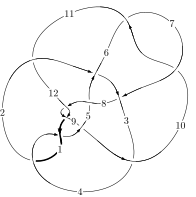
\includegraphics[width=112pt]{../../../GIT/diagram.site/Diagrams/png/1768_12a_0967.png}\\
\ \ \ A knot diagram\footnotemark}&
\allowdisplaybreaks
\textbf{Linearized knot diagam} \\
\cline{2-2}
 &
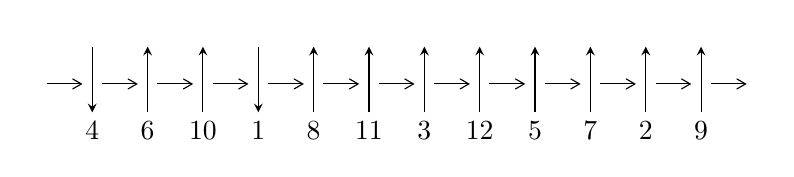
\begin{tikzpicture}[x=20pt, y=17pt]
	% nodes
	\node (C0) at (0, 0) {};
	\node (C1) at (1, 0) {};
	\node (C1U) at (1, +1) {};
	\node (C1D) at (1, -1) {4};

	\node (C2) at (2, 0) {};
	\node (C2U) at (2, +1) {};
	\node (C2D) at (2, -1) {6};

	\node (C3) at (3, 0) {};
	\node (C3U) at (3, +1) {};
	\node (C3D) at (3, -1) {10};

	\node (C4) at (4, 0) {};
	\node (C4U) at (4, +1) {};
	\node (C4D) at (4, -1) {1};

	\node (C5) at (5, 0) {};
	\node (C5U) at (5, +1) {};
	\node (C5D) at (5, -1) {8};

	\node (C6) at (6, 0) {};
	\node (C6U) at (6, +1) {};
	\node (C6D) at (6, -1) {11};

	\node (C7) at (7, 0) {};
	\node (C7U) at (7, +1) {};
	\node (C7D) at (7, -1) {3};

	\node (C8) at (8, 0) {};
	\node (C8U) at (8, +1) {};
	\node (C8D) at (8, -1) {12};

	\node (C9) at (9, 0) {};
	\node (C9U) at (9, +1) {};
	\node (C9D) at (9, -1) {5};

	\node (C10) at (10, 0) {};
	\node (C10U) at (10, +1) {};
	\node (C10D) at (10, -1) {7};

	\node (C11) at (11, 0) {};
	\node (C11U) at (11, +1) {};
	\node (C11D) at (11, -1) {2};

	\node (C12) at (12, 0) {};
	\node (C12U) at (12, +1) {};
	\node (C12D) at (12, -1) {9};
	\node (C13) at (13, 0) {};

	% arrows
	\draw[->,>={angle 60}]
	(C0) edge (C1) (C1) edge (C2) (C2) edge (C3) (C3) edge (C4) (C4) edge (C5) (C5) edge (C6) (C6) edge (C7) (C7) edge (C8) (C8) edge (C9) (C9) edge (C10) (C10) edge (C11) (C11) edge (C12) (C12) edge (C13) ;	\draw[->,>=stealth]
	(C1U) edge (C1D) (C2D) edge (C2U) (C3D) edge (C3U) (C4U) edge (C4D) (C5D) edge (C5U) (C6D) edge (C6U) (C7D) edge (C7U) (C8D) edge (C8U) (C9D) edge (C9U) (C10D) edge (C10U) (C11D) edge (C11U) (C12D) edge (C12U) ;
	\end{tikzpicture} \\
\hhline{~~} \\& 
\textbf{Solving Sequence} \\ \cline{2-2} 
 &
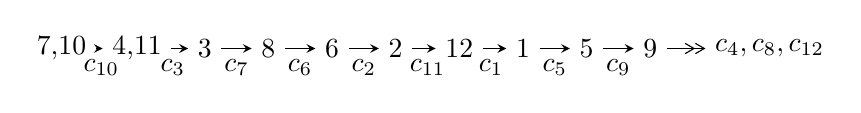
\begin{tikzpicture}[x=23pt, y=7pt]
	% node
	\node (A0) at (-1/8, 0) {7,10};
	\node (A1) at (17/16, 0) {4,11};
	\node (A2) at (17/8, 0) {3};
	\node (A3) at (25/8, 0) {8};
	\node (A4) at (33/8, 0) {6};
	\node (A5) at (41/8, 0) {2};
	\node (A6) at (49/8, 0) {12};
	\node (A7) at (57/8, 0) {1};
	\node (A8) at (65/8, 0) {5};
	\node (A9) at (73/8, 0) {9};
	\node (C1) at (1/2, -1) {$c_{10}$};
	\node (C2) at (13/8, -1) {$c_{3}$};
	\node (C3) at (21/8, -1) {$c_{7}$};
	\node (C4) at (29/8, -1) {$c_{6}$};
	\node (C5) at (37/8, -1) {$c_{2}$};
	\node (C6) at (45/8, -1) {$c_{11}$};
	\node (C7) at (53/8, -1) {$c_{1}$};
	\node (C8) at (61/8, -1) {$c_{5}$};
	\node (C9) at (69/8, -1) {$c_{9}$};
	\node (A10) at (11, 0) {$c_{4},c_{8},c_{12}$};

	% edge
	\draw[->,>=stealth]	
	(A0) edge (A1) (A1) edge (A2) (A2) edge (A3) (A3) edge (A4) (A4) edge (A5) (A5) edge (A6) (A6) edge (A7) (A7) edge (A8) (A8) edge (A9) ;
	\draw[->>,>={angle 60}]	
	(A9) edge (A10);
\end{tikzpicture} \\ 

\end{tabular} \\

\footnotetext{
The image of knot diagram is generated by the software ``\textbf{Draw programme}" developed by Andrew Bartholomew(\url{http://www.layer8.co.uk/maths/draw/index.htm\#Running-draw}), where we modified some parts for our purpose(\url{https://github.com/CATsTAILs/LinksPainter}).
}\phantom \\ \newline 
\centering \textbf{Ideals for irreducible components\footnotemark of $X_{\text{par}}$} 
 
\begin{align*}
I^u_{1}&=\langle 
-4.27600\times10^{875} u^{169}+7.13513\times10^{875} u^{168}+\cdots+1.33107\times10^{876} b+1.90372\times10^{875},\\
\phantom{I^u_{1}}&\phantom{= \langle  }1.44711\times10^{876} u^{169}-1.04949\times10^{877} u^{168}+\cdots+1.33107\times10^{876} a-2.30300\times10^{877},\\
\phantom{I^u_{1}}&\phantom{= \langle  }u^{170}-5 u^{169}+\cdots-29 u-1\rangle \\
I^u_{2}&=\langle 
3.48049\times10^{36} u^{43}-2.69494\times10^{36} u^{42}+\cdots+3.27331\times10^{36} b-1.51928\times10^{37},\\
\phantom{I^u_{2}}&\phantom{= \langle  }-1.62441\times10^{37} u^{43}-4.60073\times10^{35} u^{42}+\cdots+3.27331\times10^{36} a+6.85745\times10^{37},\\
\phantom{I^u_{2}}&\phantom{= \langle  }u^{44}+12 u^{42}+\cdots-6 u+1\rangle \\
\\
\end{align*}
\raggedright * 2 irreducible components of $\dim_{\mathbb{C}}=0$, with total 214 representations.\\
\footnotetext{All coefficients of polynomials are rational numbers. But the coefficients are sometimes approximated in decimal forms when there is not enough margin.}
\newpage
\renewcommand{\arraystretch}{1}
\centering \section*{I. $I^u_{1}= \langle -4.28\times10^{875} u^{169}+7.14\times10^{875} u^{168}+\cdots+1.33\times10^{876} b+1.90\times10^{875},\;1.45\times10^{876} u^{169}-1.05\times10^{877} u^{168}+\cdots+1.33\times10^{876} a-2.30\times10^{877},\;u^{170}-5 u^{169}+\cdots-29 u-1 \rangle$}
\flushleft \textbf{(i) Arc colorings}\\
\begin{tabular}{m{7pt} m{180pt} m{7pt} m{180pt} }
\flushright $a_{7}=$&$\begin{pmatrix}0\\u\end{pmatrix}$ \\
\flushright $a_{10}=$&$\begin{pmatrix}1\\0\end{pmatrix}$ \\
\flushright $a_{4}=$&$\begin{pmatrix}-1.08718 u^{169}+7.88454 u^{168}+\cdots+517.582 u+17.3019\\0.321246 u^{169}-0.536045 u^{168}+\cdots-14.0802 u-0.143022\end{pmatrix}$ \\
\flushright $a_{11}=$&$\begin{pmatrix}1\\- u^2\end{pmatrix}$ \\
\flushright $a_{3}=$&$\begin{pmatrix}-1.40843 u^{169}+8.42059 u^{168}+\cdots+531.663 u+17.4449\\0.321246 u^{169}-0.536045 u^{168}+\cdots-14.0802 u-0.143022\end{pmatrix}$ \\
\flushright $a_{8}=$&$\begin{pmatrix}-4.45236 u^{169}+19.7302 u^{168}+\cdots+844.035 u+32.1285\\-0.329848 u^{169}+0.912181 u^{168}+\cdots-39.0468 u-1.00358\end{pmatrix}$ \\
\flushright $a_{6}=$&$\begin{pmatrix}- u\\u^3+u\end{pmatrix}$ \\
\flushright $a_{2}=$&$\begin{pmatrix}-1.32991 u^{169}+9.02243 u^{168}+\cdots+511.041 u+16.6683\\0.397065 u^{169}-0.699324 u^{168}+\cdots-22.3763 u-0.360872\end{pmatrix}$ \\
\flushright $a_{12}=$&$\begin{pmatrix}2.70091 u^{169}-13.9853 u^{168}+\cdots+148.112 u+18.0000\\0.336931 u^{169}-1.15882 u^{168}+\cdots-55.9492 u-2.40158\end{pmatrix}$ \\
\flushright $a_{1}=$&$\begin{pmatrix}3.26780 u^{169}-15.9430 u^{168}+\cdots-576.334 u-22.1229\\-0.120267 u^{169}+1.13510 u^{168}+\cdots+34.2078 u+1.35183\end{pmatrix}$ \\
\flushright $a_{5}=$&$\begin{pmatrix}-0.764452 u^{169}+7.07131 u^{168}+\cdots+110.737 u-7.10687\\-0.0387726 u^{169}+1.38458 u^{168}+\cdots-18.0724 u+0.468304\end{pmatrix}$ \\
\flushright $a_{9}=$&$\begin{pmatrix}-2.39912 u^{169}+10.5574 u^{168}+\cdots+460.962 u+5.96555\\0.423558 u^{169}-2.34133 u^{168}+\cdots-4.08119 u+0.413028\end{pmatrix}$\\&\end{tabular}
\flushleft \textbf{(ii) Obstruction class $= -1$}\\~\\
\flushleft \textbf{(iii) Cusp Shapes $= -5.47805 u^{169}+31.7197 u^{168}+\cdots+153.364 u+10.6916$}\\~\\
\newpage\renewcommand{\arraystretch}{1}
\flushleft \textbf{(iv) u-Polynomials at the component}\newline \\
\begin{tabular}{m{50pt}|m{274pt}}
Crossings & \hspace{64pt}u-Polynomials at each crossing \\
\hline $$\begin{aligned}c_{1},c_{4}\end{aligned}$$&$\begin{aligned}
&u^{170}+8 u^{169}+\cdots-9499014 u+769055
\end{aligned}$\\
\hline $$\begin{aligned}c_{2}\end{aligned}$$&$\begin{aligned}
&u^{170}-9 u^{169}+\cdots-9312096 u+1274848
\end{aligned}$\\
\hline $$\begin{aligned}c_{3}\end{aligned}$$&$\begin{aligned}
&u^{170}+u^{169}+\cdots-1786148797 u-5447052019
\end{aligned}$\\
\hline $$\begin{aligned}c_{5}\end{aligned}$$&$\begin{aligned}
&u^{170}+13 u^{169}+\cdots+2237637 u+300169
\end{aligned}$\\
\hline $$\begin{aligned}c_{6},c_{10}\end{aligned}$$&$\begin{aligned}
&u^{170}-5 u^{169}+\cdots-29 u-1
\end{aligned}$\\
\hline $$\begin{aligned}c_{7}\end{aligned}$$&$\begin{aligned}
&u^{170}+3 u^{169}+\cdots-241024421 u+11830141
\end{aligned}$\\
\hline $$\begin{aligned}c_{8},c_{12}\end{aligned}$$&$\begin{aligned}
&u^{170}+u^{169}+\cdots+71528 u-163159
\end{aligned}$\\
\hline $$\begin{aligned}c_{9}\end{aligned}$$&$\begin{aligned}
&u^{170}-3 u^{169}+\cdots-10173208 u-3146921
\end{aligned}$\\
\hline $$\begin{aligned}c_{11}\end{aligned}$$&$\begin{aligned}
&u^{170}+12 u^{169}+\cdots-16844439 u+2548801
\end{aligned}$\\
\hline
\end{tabular}\\~\\
\newpage\renewcommand{\arraystretch}{1}
\flushleft \textbf{(v) Riley Polynomials at the component}\newline \\
\begin{tabular}{m{50pt}|m{274pt}}
Crossings & \hspace{64pt}Riley Polynomials at each crossing \\
\hline $$\begin{aligned}c_{1},c_{4}\end{aligned}$$&$\begin{aligned}
&y^{170}+124 y^{169}+\cdots-57608321480486 y+591445593025
\end{aligned}$\\
\hline $$\begin{aligned}c_{2}\end{aligned}$$&$\begin{aligned}
&y^{170}+41 y^{169}+\cdots+85496782077440 y+1625237423104
\end{aligned}$\\
\hline $$\begin{aligned}c_{3}\end{aligned}$$&$\begin{aligned}
&y^{170}+89 y^{169}+\cdots+1.51\times10^{21} y+2.97\times10^{19}
\end{aligned}$\\
\hline $$\begin{aligned}c_{5}\end{aligned}$$&$\begin{aligned}
&y^{170}+43 y^{169}+\cdots+3115277640751 y+90101428561
\end{aligned}$\\
\hline $$\begin{aligned}c_{6},c_{10}\end{aligned}$$&$\begin{aligned}
&y^{170}+113 y^{169}+\cdots+167 y+1
\end{aligned}$\\
\hline $$\begin{aligned}c_{7}\end{aligned}$$&$\begin{aligned}
&y^{170}+63 y^{169}+\cdots-8243419434057653 y+139952236079881
\end{aligned}$\\
\hline $$\begin{aligned}c_{8},c_{12}\end{aligned}$$&$\begin{aligned}
&y^{170}-133 y^{169}+\cdots-836359475222 y+26620859281
\end{aligned}$\\
\hline $$\begin{aligned}c_{9}\end{aligned}$$&$\begin{aligned}
&y^{170}-35 y^{169}+\cdots+110086202897966 y+9903111780241
\end{aligned}$\\
\hline $$\begin{aligned}c_{11}\end{aligned}$$&$\begin{aligned}
&y^{170}+56 y^{169}+\cdots+3101150912137203 y+6496386537601
\end{aligned}$\\
\hline
\end{tabular}\\~\\
\newpage\flushleft \textbf{(vi) Complex Volumes and Cusp Shapes}
$$\begin{array}{c|c|c}  
\text{Solutions to }I^u_{1}& \I (\text{vol} + \sqrt{-1}CS) & \text{Cusp shape}\\
 \hline 
\begin{aligned}
u &= -0.358984 + 0.938128 I \\
a &= \phantom{-}0.87626 + 1.72346 I \\
b &= -0.608562 + 0.995414 I\end{aligned}
 & \phantom{-}3.07880 - 5.00603 I & \phantom{-0.000000 } 0 \\ \hline\begin{aligned}
u &= -0.358984 - 0.938128 I \\
a &= \phantom{-}0.87626 - 1.72346 I \\
b &= -0.608562 - 0.995414 I\end{aligned}
 & \phantom{-}3.07880 + 5.00603 I & \phantom{-0.000000 } 0 \\ \hline\begin{aligned}
u &= \phantom{-}0.149489 + 0.981290 I \\
a &= -0.39622 + 2.63386 I \\
b &= \phantom{-}0.171353 + 1.173240 I\end{aligned}
 & \phantom{-}3.11257 + 2.64464 I & \phantom{-0.000000 } 0 \\ \hline\begin{aligned}
u &= \phantom{-}0.149489 - 0.981290 I \\
a &= -0.39622 - 2.63386 I \\
b &= \phantom{-}0.171353 - 1.173240 I\end{aligned}
 & \phantom{-}3.11257 - 2.64464 I & \phantom{-0.000000 } 0 \\ \hline\begin{aligned}
u &= -0.894429 + 0.397266 I \\
a &= \phantom{-}0.155099 - 0.844007 I \\
b &= \phantom{-}0.935844 - 0.241800 I\end{aligned}
 & \phantom{-}9.21419 - 5.10834 I & \phantom{-0.000000 } 0 \\ \hline\begin{aligned}
u &= -0.894429 - 0.397266 I \\
a &= \phantom{-}0.155099 + 0.844007 I \\
b &= \phantom{-}0.935844 + 0.241800 I\end{aligned}
 & \phantom{-}9.21419 + 5.10834 I & \phantom{-0.000000 } 0 \\ \hline\begin{aligned}
u &= \phantom{-}0.351933 + 0.905492 I \\
a &= \phantom{-}1.35732 - 0.46163 I \\
b &= -0.749929 - 0.904345 I\end{aligned}
 & \phantom{-}4.26036 + 9.83244 I & \phantom{-0.000000 } 0 \\ \hline\begin{aligned}
u &= \phantom{-}0.351933 - 0.905492 I \\
a &= \phantom{-}1.35732 + 0.46163 I \\
b &= -0.749929 + 0.904345 I\end{aligned}
 & \phantom{-}4.26036 - 9.83244 I & \phantom{-0.000000 } 0 \\ \hline\begin{aligned}
u &= -0.959787 + 0.021614 I \\
a &= \phantom{-}0.356042 + 0.363318 I \\
b &= -0.041148 - 0.436442 I\end{aligned}
 & \phantom{-}0.36103 + 3.02788 I & \phantom{-0.000000 } 0 \\ \hline\begin{aligned}
u &= -0.959787 - 0.021614 I \\
a &= \phantom{-}0.356042 - 0.363318 I \\
b &= -0.041148 + 0.436442 I\end{aligned}
 & \phantom{-}0.36103 - 3.02788 I & \phantom{-0.000000 } 0\\
 \hline 
 \end{array}$$\newpage$$\begin{array}{c|c|c}  
\text{Solutions to }I^u_{1}& \I (\text{vol} + \sqrt{-1}CS) & \text{Cusp shape}\\
 \hline 
\begin{aligned}
u &= \phantom{-}0.905359 + 0.519808 I \\
a &= -0.211162 + 1.148670 I \\
b &= \phantom{-}0.345219 + 1.235090 I\end{aligned}
 & \phantom{-}5.79176 - 0.63772 I & \phantom{-0.000000 } 0 \\ \hline\begin{aligned}
u &= \phantom{-}0.905359 - 0.519808 I \\
a &= -0.211162 - 1.148670 I \\
b &= \phantom{-}0.345219 - 1.235090 I\end{aligned}
 & \phantom{-}5.79176 + 0.63772 I & \phantom{-0.000000 } 0 \\ \hline\begin{aligned}
u &= -1.041260 + 0.162137 I \\
a &= -0.195765 - 0.371659 I \\
b &= \phantom{-}0.491730 - 1.137210 I\end{aligned}
 & -3.39653 - 4.01857 I & \phantom{-0.000000 } 0 \\ \hline\begin{aligned}
u &= -1.041260 - 0.162137 I \\
a &= -0.195765 + 0.371659 I \\
b &= \phantom{-}0.491730 + 1.137210 I\end{aligned}
 & -3.39653 + 4.01857 I & \phantom{-0.000000 } 0 \\ \hline\begin{aligned}
u &= -0.129388 + 1.047410 I \\
a &= -0.203586 - 0.159028 I \\
b &= \phantom{-}0.728530 + 0.259066 I\end{aligned}
 & \phantom{-}1.56798 - 2.38640 I & \phantom{-0.000000 } 0 \\ \hline\begin{aligned}
u &= -0.129388 - 1.047410 I \\
a &= -0.203586 + 0.159028 I \\
b &= \phantom{-}0.728530 - 0.259066 I\end{aligned}
 & \phantom{-}1.56798 + 2.38640 I & \phantom{-0.000000 } 0 \\ \hline\begin{aligned}
u &= -0.086351 + 1.062530 I \\
a &= \phantom{-}0.86211 - 2.82247 I \\
b &= \phantom{-}0.423310 - 1.299350 I\end{aligned}
 & \phantom{-}3.02815 + 2.97469 I & \phantom{-0.000000 } 0 \\ \hline\begin{aligned}
u &= -0.086351 - 1.062530 I \\
a &= \phantom{-}0.86211 + 2.82247 I \\
b &= \phantom{-}0.423310 + 1.299350 I\end{aligned}
 & \phantom{-}3.02815 - 2.97469 I & \phantom{-0.000000 } 0 \\ \hline\begin{aligned}
u &= \phantom{-}0.654950 + 0.662580 I \\
a &= \phantom{-}0.663710 + 0.797078 I \\
b &= \phantom{-}0.303235 - 0.747358 I\end{aligned}
 & \phantom{-}4.97571 - 5.72324 I & \phantom{-0.000000 } 0 \\ \hline\begin{aligned}
u &= \phantom{-}0.654950 - 0.662580 I \\
a &= \phantom{-}0.663710 - 0.797078 I \\
b &= \phantom{-}0.303235 + 0.747358 I\end{aligned}
 & \phantom{-}4.97571 + 5.72324 I & \phantom{-0.000000 } 0\\
 \hline 
 \end{array}$$\newpage$$\begin{array}{c|c|c}  
\text{Solutions to }I^u_{1}& \I (\text{vol} + \sqrt{-1}CS) & \text{Cusp shape}\\
 \hline 
\begin{aligned}
u &= -0.363380 + 1.025540 I \\
a &= -1.66170 + 0.71346 I \\
b &= -2.25117 + 0.25267 I\end{aligned}
 & \phantom{-}4.44981 - 10.87120 I & \phantom{-0.000000 } 0 \\ \hline\begin{aligned}
u &= -0.363380 - 1.025540 I \\
a &= -1.66170 - 0.71346 I \\
b &= -2.25117 - 0.25267 I\end{aligned}
 & \phantom{-}4.44981 + 10.87120 I & \phantom{-0.000000 } 0 \\ \hline\begin{aligned}
u &= -0.685164 + 0.600930 I \\
a &= \phantom{-}0.131451 - 0.227585 I \\
b &= \phantom{-}0.598615 + 0.763837 I\end{aligned}
 & \phantom{-}4.07366 + 0.83692 I & \phantom{-0.000000 } 0 \\ \hline\begin{aligned}
u &= -0.685164 - 0.600930 I \\
a &= \phantom{-}0.131451 + 0.227585 I \\
b &= \phantom{-}0.598615 - 0.763837 I\end{aligned}
 & \phantom{-}4.07366 - 0.83692 I & \phantom{-0.000000 } 0 \\ \hline\begin{aligned}
u &= -1.076660 + 0.171449 I \\
a &= -0.0898171 + 0.0136149 I \\
b &= \phantom{-}0.124258 + 1.042590 I\end{aligned}
 & \phantom{-}0.73430 + 3.64814 I & \phantom{-0.000000 } 0 \\ \hline\begin{aligned}
u &= -1.076660 - 0.171449 I \\
a &= -0.0898171 - 0.0136149 I \\
b &= \phantom{-}0.124258 - 1.042590 I\end{aligned}
 & \phantom{-}0.73430 - 3.64814 I & \phantom{-0.000000 } 0 \\ \hline\begin{aligned}
u &= \phantom{-}1.073740 + 0.190083 I \\
a &= \phantom{-}0.202327 - 0.371251 I \\
b &= -0.579160 - 0.999760 I\end{aligned}
 & -0.17316 + 8.52716 I & \phantom{-0.000000 } 0 \\ \hline\begin{aligned}
u &= \phantom{-}1.073740 - 0.190083 I \\
a &= \phantom{-}0.202327 + 0.371251 I \\
b &= -0.579160 + 0.999760 I\end{aligned}
 & -0.17316 - 8.52716 I & \phantom{-0.000000 } 0 \\ \hline\begin{aligned}
u &= \phantom{-}0.881440 + 0.189216 I \\
a &= -0.762298 - 0.049409 I \\
b &= -1.23696 + 1.13928 I\end{aligned}
 & \phantom{-}3.58537 + 1.10845 I & \phantom{-0.000000 } 0 \\ \hline\begin{aligned}
u &= \phantom{-}0.881440 - 0.189216 I \\
a &= -0.762298 + 0.049409 I \\
b &= -1.23696 - 1.13928 I\end{aligned}
 & \phantom{-}3.58537 - 1.10845 I & \phantom{-0.000000 } 0\\
 \hline 
 \end{array}$$\newpage$$\begin{array}{c|c|c}  
\text{Solutions to }I^u_{1}& \I (\text{vol} + \sqrt{-1}CS) & \text{Cusp shape}\\
 \hline 
\begin{aligned}
u &= \phantom{-}0.792880 + 0.428256 I \\
a &= -0.564492 - 0.509799 I \\
b &= -1.036170 + 0.406270 I\end{aligned}
 & \phantom{-}3.41659 + 0.91213 I & \phantom{-0.000000 } 0 \\ \hline\begin{aligned}
u &= \phantom{-}0.792880 - 0.428256 I \\
a &= -0.564492 + 0.509799 I \\
b &= -1.036170 - 0.406270 I\end{aligned}
 & \phantom{-}3.41659 - 0.91213 I & \phantom{-0.000000 } 0 \\ \hline\begin{aligned}
u &= -0.272810 + 1.076190 I \\
a &= -0.37197 - 1.70523 I \\
b &= \phantom{-}0.32902 - 1.56267 I\end{aligned}
 & -4.15359 - 1.41570 I & \phantom{-0.000000 } 0 \\ \hline\begin{aligned}
u &= -0.272810 - 1.076190 I \\
a &= -0.37197 + 1.70523 I \\
b &= \phantom{-}0.32902 + 1.56267 I\end{aligned}
 & -4.15359 + 1.41570 I & \phantom{-0.000000 } 0 \\ \hline\begin{aligned}
u &= \phantom{-}0.391618 + 1.039960 I \\
a &= -0.04388 + 1.53153 I \\
b &= \phantom{-}0.97841 + 1.03325 I\end{aligned}
 & \phantom{-}1.46563 + 3.45220 I & \phantom{-0.000000 } 0 \\ \hline\begin{aligned}
u &= \phantom{-}0.391618 - 1.039960 I \\
a &= -0.04388 - 1.53153 I \\
b &= \phantom{-}0.97841 - 1.03325 I\end{aligned}
 & \phantom{-}1.46563 - 3.45220 I & \phantom{-0.000000 } 0 \\ \hline\begin{aligned}
u &= \phantom{-}0.086089 + 1.113660 I \\
a &= -0.38989 - 2.37911 I \\
b &= -0.91963 - 1.22060 I\end{aligned}
 & -2.12231 + 1.70533 I & \phantom{-0.000000 } 0 \\ \hline\begin{aligned}
u &= \phantom{-}0.086089 - 1.113660 I \\
a &= -0.38989 + 2.37911 I \\
b &= -0.91963 + 1.22060 I\end{aligned}
 & -2.12231 - 1.70533 I & \phantom{-0.000000 } 0 \\ \hline\begin{aligned}
u &= \phantom{-}0.461621 + 1.021630 I \\
a &= -1.013880 + 0.786959 I \\
b &= -0.949096 + 0.684986 I\end{aligned}
 & \phantom{-}4.10713 + 5.60266 I & \phantom{-0.000000 } 0 \\ \hline\begin{aligned}
u &= \phantom{-}0.461621 - 1.021630 I \\
a &= -1.013880 - 0.786959 I \\
b &= -0.949096 - 0.684986 I\end{aligned}
 & \phantom{-}4.10713 - 5.60266 I & \phantom{-0.000000 } 0\\
 \hline 
 \end{array}$$\newpage$$\begin{array}{c|c|c}  
\text{Solutions to }I^u_{1}& \I (\text{vol} + \sqrt{-1}CS) & \text{Cusp shape}\\
 \hline 
\begin{aligned}
u &= -0.146778 + 1.113650 I \\
a &= -0.00568 + 2.77042 I \\
b &= -0.40913 + 2.28459 I\end{aligned}
 & -2.23788 - 5.07178 I & \phantom{-0.000000 } 0 \\ \hline\begin{aligned}
u &= -0.146778 - 1.113650 I \\
a &= -0.00568 - 2.77042 I \\
b &= -0.40913 - 2.28459 I\end{aligned}
 & -2.23788 + 5.07178 I & \phantom{-0.000000 } 0 \\ \hline\begin{aligned}
u &= \phantom{-}0.505522 + 1.010370 I \\
a &= \phantom{-}1.16249 + 1.67396 I \\
b &= \phantom{-}1.95237 + 1.03140 I\end{aligned}
 & \phantom{-}1.26931 + 3.95660 I & \phantom{-0.000000 } 0 \\ \hline\begin{aligned}
u &= \phantom{-}0.505522 - 1.010370 I \\
a &= \phantom{-}1.16249 - 1.67396 I \\
b &= \phantom{-}1.95237 - 1.03140 I\end{aligned}
 & \phantom{-}1.26931 - 3.95660 I & \phantom{-0.000000 } 0 \\ \hline\begin{aligned}
u &= -0.002446 + 1.130940 I \\
a &= \phantom{-}0.51199 - 2.17240 I \\
b &= \phantom{-}1.10202 - 1.91613 I\end{aligned}
 & -5.67349 + 0.05332 I & \phantom{-0.000000 } 0 \\ \hline\begin{aligned}
u &= -0.002446 - 1.130940 I \\
a &= \phantom{-}0.51199 + 2.17240 I \\
b &= \phantom{-}1.10202 + 1.91613 I\end{aligned}
 & -5.67349 - 0.05332 I & \phantom{-0.000000 } 0 \\ \hline\begin{aligned}
u &= -0.140161 + 1.132330 I \\
a &= -0.05789 + 1.46164 I \\
b &= \phantom{-}0.648806 + 0.874273 I\end{aligned}
 & -2.31461 - 3.55736 I & \phantom{-0.000000 } 0 \\ \hline\begin{aligned}
u &= -0.140161 - 1.132330 I \\
a &= -0.05789 - 1.46164 I \\
b &= \phantom{-}0.648806 - 0.874273 I\end{aligned}
 & -2.31461 + 3.55736 I & \phantom{-0.000000 } 0 \\ \hline\begin{aligned}
u &= -0.263762 + 1.115710 I \\
a &= -0.81839 - 1.32101 I \\
b &= \phantom{-}0.832256 - 0.841845 I\end{aligned}
 & -0.97904 - 6.10867 I & \phantom{-0.000000 } 0 \\ \hline\begin{aligned}
u &= -0.263762 - 1.115710 I \\
a &= -0.81839 + 1.32101 I \\
b &= \phantom{-}0.832256 + 0.841845 I\end{aligned}
 & -0.97904 + 6.10867 I & \phantom{-0.000000 } 0\\
 \hline 
 \end{array}$$\newpage$$\begin{array}{c|c|c}  
\text{Solutions to }I^u_{1}& \I (\text{vol} + \sqrt{-1}CS) & \text{Cusp shape}\\
 \hline 
\begin{aligned}
u &= -0.133321 + 1.146710 I \\
a &= \phantom{-}1.46605 - 2.90758 I \\
b &= \phantom{-}0.466582 - 0.741270 I\end{aligned}
 & \phantom{-}1.34073 - 10.06810 I & \phantom{-0.000000 } 0 \\ \hline\begin{aligned}
u &= -0.133321 - 1.146710 I \\
a &= \phantom{-}1.46605 + 2.90758 I \\
b &= \phantom{-}0.466582 + 0.741270 I\end{aligned}
 & \phantom{-}1.34073 + 10.06810 I & \phantom{-0.000000 } 0 \\ \hline\begin{aligned}
u &= -0.482607 + 1.049530 I \\
a &= -0.583589 + 0.577217 I \\
b &= -1.303960 + 0.237660 I\end{aligned}
 & \phantom{-}7.14469 + 0.17226 I & \phantom{-0.000000 } 0 \\ \hline\begin{aligned}
u &= -0.482607 - 1.049530 I \\
a &= -0.583589 - 0.577217 I \\
b &= -1.303960 - 0.237660 I\end{aligned}
 & \phantom{-}7.14469 - 0.17226 I & \phantom{-0.000000 } 0 \\ \hline\begin{aligned}
u &= -0.031379 + 1.154950 I \\
a &= -1.20303 + 2.28802 I \\
b &= \phantom{-}0.144926 + 0.792707 I\end{aligned}
 & -3.86382 - 3.91324 I & \phantom{-0.000000 } 0 \\ \hline\begin{aligned}
u &= -0.031379 - 1.154950 I \\
a &= -1.20303 - 2.28802 I \\
b &= \phantom{-}0.144926 - 0.792707 I\end{aligned}
 & -3.86382 + 3.91324 I & \phantom{-0.000000 } 0 \\ \hline\begin{aligned}
u &= -0.060169 + 1.170230 I \\
a &= \phantom{-}1.73726 + 2.16803 I \\
b &= -0.071987 + 0.827595 I\end{aligned}
 & -6.51258 - 1.32939 I & \phantom{-0.000000 } 0 \\ \hline\begin{aligned}
u &= -0.060169 - 1.170230 I \\
a &= \phantom{-}1.73726 - 2.16803 I \\
b &= -0.071987 - 0.827595 I\end{aligned}
 & -6.51258 + 1.32939 I & \phantom{-0.000000 } 0 \\ \hline\begin{aligned}
u &= -0.689189 + 0.458239 I \\
a &= \phantom{-}0.76961 - 1.77227 I \\
b &= \phantom{-}1.57785 - 0.55541 I\end{aligned}
 & \phantom{-}6.16352 + 6.82205 I & \phantom{-0.000000 } 0 \\ \hline\begin{aligned}
u &= -0.689189 - 0.458239 I \\
a &= \phantom{-}0.76961 + 1.77227 I \\
b &= \phantom{-}1.57785 + 0.55541 I\end{aligned}
 & \phantom{-}6.16352 - 6.82205 I & \phantom{-0.000000 } 0\\
 \hline 
 \end{array}$$\newpage$$\begin{array}{c|c|c}  
\text{Solutions to }I^u_{1}& \I (\text{vol} + \sqrt{-1}CS) & \text{Cusp shape}\\
 \hline 
\begin{aligned}
u &= -1.177070 + 0.017293 I \\
a &= -0.356734 - 0.365238 I \\
b &= -0.93177 - 1.22908 I\end{aligned}
 & -0.81185 + 8.17295 I & \phantom{-0.000000 } 0 \\ \hline\begin{aligned}
u &= -1.177070 - 0.017293 I \\
a &= -0.356734 + 0.365238 I \\
b &= -0.93177 + 1.22908 I\end{aligned}
 & -0.81185 - 8.17295 I & \phantom{-0.000000 } 0 \\ \hline\begin{aligned}
u &= \phantom{-}1.177000 + 0.081728 I \\
a &= \phantom{-}0.015198 + 0.153559 I \\
b &= -0.153265 + 0.887761 I\end{aligned}
 & \phantom{-}0.10469 - 2.34643 I & \phantom{-0.000000 } 0 \\ \hline\begin{aligned}
u &= \phantom{-}1.177000 - 0.081728 I \\
a &= \phantom{-}0.015198 - 0.153559 I \\
b &= -0.153265 - 0.887761 I\end{aligned}
 & \phantom{-}0.10469 + 2.34643 I & \phantom{-0.000000 } 0 \\ \hline\begin{aligned}
u &= \phantom{-}0.141190 + 1.172410 I \\
a &= \phantom{-}0.681885 + 0.688923 I \\
b &= -0.590588 + 0.473327 I\end{aligned}
 & -0.10416 + 4.97008 I & \phantom{-0.000000 } 0 \\ \hline\begin{aligned}
u &= \phantom{-}0.141190 - 1.172410 I \\
a &= \phantom{-}0.681885 - 0.688923 I \\
b &= -0.590588 - 0.473327 I\end{aligned}
 & -0.10416 - 4.97008 I & \phantom{-0.000000 } 0 \\ \hline\begin{aligned}
u &= \phantom{-}1.181030 + 0.017013 I \\
a &= \phantom{-}0.176539 + 0.377081 I \\
b &= \phantom{-}0.80489 + 1.21474 I\end{aligned}
 & \phantom{-}3.9574 + 14.5268 I & \phantom{-0.000000 } 0 \\ \hline\begin{aligned}
u &= \phantom{-}1.181030 - 0.017013 I \\
a &= \phantom{-}0.176539 - 0.377081 I \\
b &= \phantom{-}0.80489 - 1.21474 I\end{aligned}
 & \phantom{-}3.9574 - 14.5268 I & \phantom{-0.000000 } 0 \\ \hline\begin{aligned}
u &= -0.143324 + 0.804171 I \\
a &= \phantom{-}1.278900 + 0.351900 I \\
b &= \phantom{-}1.42970 - 0.35652 I\end{aligned}
 & -0.45328 - 1.51618 I & \phantom{-0.000000 } 0 \\ \hline\begin{aligned}
u &= -0.143324 - 0.804171 I \\
a &= \phantom{-}1.278900 - 0.351900 I \\
b &= \phantom{-}1.42970 + 0.35652 I\end{aligned}
 & -0.45328 + 1.51618 I & \phantom{-0.000000 } 0\\
 \hline 
 \end{array}$$\newpage$$\begin{array}{c|c|c}  
\text{Solutions to }I^u_{1}& \I (\text{vol} + \sqrt{-1}CS) & \text{Cusp shape}\\
 \hline 
\begin{aligned}
u &= \phantom{-}0.006920 + 0.809989 I \\
a &= \phantom{-}0.208219 - 0.071614 I \\
b &= -0.994123 - 0.986019 I\end{aligned}
 & \phantom{-}4.07975 - 3.55082 I & \phantom{-0.000000 } 0 \\ \hline\begin{aligned}
u &= \phantom{-}0.006920 - 0.809989 I \\
a &= \phantom{-}0.208219 + 0.071614 I \\
b &= -0.994123 + 0.986019 I\end{aligned}
 & \phantom{-}4.07975 + 3.55082 I & \phantom{-0.000000 } 0 \\ \hline\begin{aligned}
u &= -0.030537 + 1.190400 I \\
a &= \phantom{-}0.082000 - 1.054390 I \\
b &= -0.500202 - 0.500794 I\end{aligned}
 & -3.34741 + 0.91547 I & \phantom{-0.000000 } 0 \\ \hline\begin{aligned}
u &= -0.030537 - 1.190400 I \\
a &= \phantom{-}0.082000 + 1.054390 I \\
b &= -0.500202 + 0.500794 I\end{aligned}
 & -3.34741 - 0.91547 I & \phantom{-0.000000 } 0 \\ \hline\begin{aligned}
u &= \phantom{-}0.012089 + 1.194870 I \\
a &= -0.55756 - 1.64583 I \\
b &= -1.27632 - 1.37676 I\end{aligned}
 & -4.50477 + 3.57230 I & \phantom{-0.000000 } 0 \\ \hline\begin{aligned}
u &= \phantom{-}0.012089 - 1.194870 I \\
a &= -0.55756 + 1.64583 I \\
b &= -1.27632 + 1.37676 I\end{aligned}
 & -4.50477 - 3.57230 I & \phantom{-0.000000 } 0 \\ \hline\begin{aligned}
u &= \phantom{-}0.523557 + 0.610774 I \\
a &= -0.1145730 - 0.0252207 I \\
b &= -0.657466 + 0.712414 I\end{aligned}
 & \phantom{-}3.87323 + 0.06583 I & \phantom{-0.000000 } 0 \\ \hline\begin{aligned}
u &= \phantom{-}0.523557 - 0.610774 I \\
a &= -0.1145730 + 0.0252207 I \\
b &= -0.657466 - 0.712414 I\end{aligned}
 & \phantom{-}3.87323 - 0.06583 I & \phantom{-0.000000 } 0 \\ \hline\begin{aligned}
u &= \phantom{-}0.155581 + 1.185740 I \\
a &= \phantom{-}0.41969 + 2.44964 I \\
b &= \phantom{-}1.01446 + 2.11185 I\end{aligned}
 & \phantom{-}0.60520 + 10.41640 I & \phantom{-0.000000 } 0 \\ \hline\begin{aligned}
u &= \phantom{-}0.155581 - 1.185740 I \\
a &= \phantom{-}0.41969 - 2.44964 I \\
b &= \phantom{-}1.01446 - 2.11185 I\end{aligned}
 & \phantom{-}0.60520 - 10.41640 I & \phantom{-0.000000 } 0\\
 \hline 
 \end{array}$$\newpage$$\begin{array}{c|c|c}  
\text{Solutions to }I^u_{1}& \I (\text{vol} + \sqrt{-1}CS) & \text{Cusp shape}\\
 \hline 
\begin{aligned}
u &= \phantom{-}1.186320 + 0.231731 I \\
a &= -0.319999 + 0.082786 I \\
b &= -0.124459 + 0.600565 I\end{aligned}
 & \phantom{-}0.47324 - 1.33934 I & \phantom{-0.000000 } 0 \\ \hline\begin{aligned}
u &= \phantom{-}1.186320 - 0.231731 I \\
a &= -0.319999 - 0.082786 I \\
b &= -0.124459 - 0.600565 I\end{aligned}
 & \phantom{-}0.47324 + 1.33934 I & \phantom{-0.000000 } 0 \\ \hline\begin{aligned}
u &= \phantom{-}0.125959 + 1.214400 I \\
a &= -1.66229 - 2.02190 I \\
b &= -0.494152 - 0.538175 I\end{aligned}
 & -4.18915 + 4.21221 I & \phantom{-0.000000 } 0 \\ \hline\begin{aligned}
u &= \phantom{-}0.125959 - 1.214400 I \\
a &= -1.66229 + 2.02190 I \\
b &= -0.494152 + 0.538175 I\end{aligned}
 & -4.18915 - 4.21221 I & \phantom{-0.000000 } 0 \\ \hline\begin{aligned}
u &= \phantom{-}0.112463 + 1.222680 I \\
a &= -0.682429 + 0.211029 I \\
b &= -1.293920 + 0.355891 I\end{aligned}
 & -4.23647 + 2.40719 I & \phantom{-0.000000 } 0 \\ \hline\begin{aligned}
u &= \phantom{-}0.112463 - 1.222680 I \\
a &= -0.682429 - 0.211029 I \\
b &= -1.293920 - 0.355891 I\end{aligned}
 & -4.23647 - 2.40719 I & \phantom{-0.000000 } 0 \\ \hline\begin{aligned}
u &= \phantom{-}0.738707 + 0.196649 I \\
a &= \phantom{-}0.363855 - 0.288314 I \\
b &= -0.146217 + 0.994810 I\end{aligned}
 & \phantom{-}1.87552 - 2.30328 I & \phantom{-0.000000 } 0 \\ \hline\begin{aligned}
u &= \phantom{-}0.738707 - 0.196649 I \\
a &= \phantom{-}0.363855 + 0.288314 I \\
b &= -0.146217 - 0.994810 I\end{aligned}
 & \phantom{-}1.87552 + 2.30328 I & \phantom{-0.000000 } 0 \\ \hline\begin{aligned}
u &= -0.169648 + 1.232630 I \\
a &= \phantom{-}0.792877 + 0.682508 I \\
b &= \phantom{-}1.31029 + 0.74185 I\end{aligned}
 & -2.63492 - 6.62405 I & \phantom{-0.000000 } 0 \\ \hline\begin{aligned}
u &= -0.169648 - 1.232630 I \\
a &= \phantom{-}0.792877 - 0.682508 I \\
b &= \phantom{-}1.31029 - 0.74185 I\end{aligned}
 & -2.63492 + 6.62405 I & \phantom{-0.000000 } 0\\
 \hline 
 \end{array}$$\newpage$$\begin{array}{c|c|c}  
\text{Solutions to }I^u_{1}& \I (\text{vol} + \sqrt{-1}CS) & \text{Cusp shape}\\
 \hline 
\begin{aligned}
u &= -0.198813 + 1.228620 I \\
a &= -0.221282 - 1.295030 I \\
b &= \phantom{-}1.028340 - 0.759335 I\end{aligned}
 & -0.67043 - 5.81168 I & \phantom{-0.000000 } 0 \\ \hline\begin{aligned}
u &= -0.198813 - 1.228620 I \\
a &= -0.221282 + 1.295030 I \\
b &= \phantom{-}1.028340 + 0.759335 I\end{aligned}
 & -0.67043 + 5.81168 I & \phantom{-0.000000 } 0 \\ \hline\begin{aligned}
u &= \phantom{-}0.257373 + 1.243960 I \\
a &= -1.39878 + 1.55383 I \\
b &= \phantom{-}0.132742 + 1.042640 I\end{aligned}
 & -1.43857 + 6.12757 I & \phantom{-0.000000 } 0 \\ \hline\begin{aligned}
u &= \phantom{-}0.257373 - 1.243960 I \\
a &= -1.39878 - 1.55383 I \\
b &= \phantom{-}0.132742 - 1.042640 I\end{aligned}
 & -1.43857 - 6.12757 I & \phantom{-0.000000 } 0 \\ \hline\begin{aligned}
u &= \phantom{-}0.702950 + 0.145538 I \\
a &= -0.210636 - 0.383777 I \\
b &= \phantom{-}0.621542 + 0.158058 I\end{aligned}
 & \phantom{-}0.339928 - 0.226718 I & \phantom{-0.000000 } 0 \\ \hline\begin{aligned}
u &= \phantom{-}0.702950 - 0.145538 I \\
a &= -0.210636 + 0.383777 I \\
b &= \phantom{-}0.621542 - 0.158058 I\end{aligned}
 & \phantom{-}0.339928 + 0.226718 I & \phantom{-0.000000 } 0 \\ \hline\begin{aligned}
u &= \phantom{-}0.257093 + 1.281870 I \\
a &= \phantom{-}0.337818 - 0.998986 I \\
b &= -0.905144 - 0.513805 I\end{aligned}
 & \phantom{-}0.56703 + 5.58880 I & \phantom{-0.000000 } 0 \\ \hline\begin{aligned}
u &= \phantom{-}0.257093 - 1.281870 I \\
a &= \phantom{-}0.337818 + 0.998986 I \\
b &= -0.905144 + 0.513805 I\end{aligned}
 & \phantom{-}0.56703 - 5.58880 I & \phantom{-0.000000 } 0 \\ \hline\begin{aligned}
u &= \phantom{-}0.089120 + 1.306080 I \\
a &= \phantom{-}0.04092 - 1.48051 I \\
b &= -0.324188 - 1.284790 I\end{aligned}
 & -3.31007 + 0.31222 I & \phantom{-0.000000 } 0 \\ \hline\begin{aligned}
u &= \phantom{-}0.089120 - 1.306080 I \\
a &= \phantom{-}0.04092 + 1.48051 I \\
b &= -0.324188 + 1.284790 I\end{aligned}
 & -3.31007 - 0.31222 I & \phantom{-0.000000 } 0\\
 \hline 
 \end{array}$$\newpage$$\begin{array}{c|c|c}  
\text{Solutions to }I^u_{1}& \I (\text{vol} + \sqrt{-1}CS) & \text{Cusp shape}\\
 \hline 
\begin{aligned}
u &= \phantom{-}0.437398 + 1.245460 I \\
a &= -0.927788 - 0.033295 I \\
b &= -0.162519 + 0.473485 I\end{aligned}
 & -2.87035 + 4.53612 I & \phantom{-0.000000 } 0 \\ \hline\begin{aligned}
u &= \phantom{-}0.437398 - 1.245460 I \\
a &= -0.927788 + 0.033295 I \\
b &= -0.162519 - 0.473485 I\end{aligned}
 & -2.87035 - 4.53612 I & \phantom{-0.000000 } 0 \\ \hline\begin{aligned}
u &= -0.124227 + 1.315620 I \\
a &= \phantom{-}0.24894 - 1.68309 I \\
b &= \phantom{-}0.059017 - 0.781041 I\end{aligned}
 & -2.98246 + 0.79000 I & \phantom{-0.000000 } 0 \\ \hline\begin{aligned}
u &= -0.124227 - 1.315620 I \\
a &= \phantom{-}0.24894 + 1.68309 I \\
b &= \phantom{-}0.059017 + 0.781041 I\end{aligned}
 & -2.98246 - 0.79000 I & \phantom{-0.000000 } 0 \\ \hline\begin{aligned}
u &= -0.670747 + 0.001839 I \\
a &= \phantom{-}0.507676 + 0.953054 I \\
b &= -0.696949 + 0.443077 I\end{aligned}
 & \phantom{-}1.35614 + 3.70926 I & \phantom{-0.000000 } 0 \\ \hline\begin{aligned}
u &= -0.670747 - 0.001839 I \\
a &= \phantom{-}0.507676 - 0.953054 I \\
b &= -0.696949 - 0.443077 I\end{aligned}
 & \phantom{-}1.35614 - 3.70926 I & \phantom{-0.000000 } 0 \\ \hline\begin{aligned}
u &= -0.576671 + 0.315628 I \\
a &= \phantom{-}0.041104 + 1.266560 I \\
b &= -0.345092 - 0.509200 I\end{aligned}
 & \phantom{-}1.44984 + 2.85698 I & \phantom{-0.000000 } 0 \\ \hline\begin{aligned}
u &= -0.576671 - 0.315628 I \\
a &= \phantom{-}0.041104 - 1.266560 I \\
b &= -0.345092 + 0.509200 I\end{aligned}
 & \phantom{-}1.44984 - 2.85698 I & \phantom{-0.000000 } 0 \\ \hline\begin{aligned}
u &= -0.393385 + 1.302880 I \\
a &= -0.30569 - 1.41517 I \\
b &= \phantom{-}0.35923 - 1.37450 I\end{aligned}
 & -4.24700 - 1.20015 I & \phantom{-0.000000 } 0 \\ \hline\begin{aligned}
u &= -0.393385 - 1.302880 I \\
a &= -0.30569 + 1.41517 I \\
b &= \phantom{-}0.35923 + 1.37450 I\end{aligned}
 & -4.24700 + 1.20015 I & \phantom{-0.000000 } 0\\
 \hline 
 \end{array}$$\newpage$$\begin{array}{c|c|c}  
\text{Solutions to }I^u_{1}& \I (\text{vol} + \sqrt{-1}CS) & \text{Cusp shape}\\
 \hline 
\begin{aligned}
u &= \phantom{-}1.367910 + 0.102452 I \\
a &= \phantom{-}0.347756 - 1.202100 I \\
b &= \phantom{-}0.42962 - 2.11328 I\end{aligned}
 & \phantom{-}4.32919 + 0.16885 I & \phantom{-0.000000 } 0 \\ \hline\begin{aligned}
u &= \phantom{-}1.367910 - 0.102452 I \\
a &= \phantom{-}0.347756 + 1.202100 I \\
b &= \phantom{-}0.42962 + 2.11328 I\end{aligned}
 & \phantom{-}4.32919 - 0.16885 I & \phantom{-0.000000 } 0 \\ \hline\begin{aligned}
u &= -0.590101 + 1.246510 I \\
a &= -0.190565 + 1.225250 I \\
b &= -0.700767 + 1.215870 I\end{aligned}
 & -3.13756 - 2.07733 I & \phantom{-0.000000 } 0 \\ \hline\begin{aligned}
u &= -0.590101 - 1.246510 I \\
a &= -0.190565 - 1.225250 I \\
b &= -0.700767 - 1.215870 I\end{aligned}
 & -3.13756 + 2.07733 I & \phantom{-0.000000 } 0 \\ \hline\begin{aligned}
u &= -0.608738\phantom{ +0.000000I} \\
a &= \phantom{-}1.17642\phantom{ +0.000000I} \\
b &= -0.588708\phantom{ +0.000000I}\end{aligned}
 & \phantom{-}4.90876\phantom{ +0.000000I} & \phantom{-0.000000 } 0 \\ \hline\begin{aligned}
u &= -0.46986 + 1.33718 I \\
a &= -0.234856 - 0.808441 I \\
b &= \phantom{-}0.726013 - 0.746689 I\end{aligned}
 & -3.85896 - 8.23184 I & \phantom{-0.000000 } 0 \\ \hline\begin{aligned}
u &= -0.46986 - 1.33718 I \\
a &= -0.234856 + 0.808441 I \\
b &= \phantom{-}0.726013 + 0.746689 I\end{aligned}
 & -3.85896 + 8.23184 I & \phantom{-0.000000 } 0 \\ \hline\begin{aligned}
u &= \phantom{-}0.50295 + 1.33882 I \\
a &= \phantom{-}1.64814 - 1.25440 I \\
b &= \phantom{-}0.40678 - 1.49148 I\end{aligned}
 & -0.87982 + 6.10551 I & \phantom{-0.000000 } 0 \\ \hline\begin{aligned}
u &= \phantom{-}0.50295 - 1.33882 I \\
a &= \phantom{-}1.64814 + 1.25440 I \\
b &= \phantom{-}0.40678 + 1.49148 I\end{aligned}
 & -0.87982 - 6.10551 I & \phantom{-0.000000 } 0 \\ \hline\begin{aligned}
u &= \phantom{-}0.34904 + 1.40048 I \\
a &= -1.32223 + 1.85888 I \\
b &= -0.03816 + 1.46590 I\end{aligned}
 & -1.54791 + 6.03526 I & \phantom{-0.000000 } 0\\
 \hline 
 \end{array}$$\newpage$$\begin{array}{c|c|c}  
\text{Solutions to }I^u_{1}& \I (\text{vol} + \sqrt{-1}CS) & \text{Cusp shape}\\
 \hline 
\begin{aligned}
u &= \phantom{-}0.34904 - 1.40048 I \\
a &= -1.32223 - 1.85888 I \\
b &= -0.03816 - 1.46590 I\end{aligned}
 & -1.54791 - 6.03526 I & \phantom{-0.000000 } 0 \\ \hline\begin{aligned}
u &= \phantom{-}0.42027 + 1.38795 I \\
a &= \phantom{-}0.204470 - 1.059950 I \\
b &= -0.653211 - 0.882158 I\end{aligned}
 & -4.86374 + 3.88643 I & \phantom{-0.000000 } 0 \\ \hline\begin{aligned}
u &= \phantom{-}0.42027 - 1.38795 I \\
a &= \phantom{-}0.204470 + 1.059950 I \\
b &= -0.653211 + 0.882158 I\end{aligned}
 & -4.86374 - 3.88643 I & \phantom{-0.000000 } 0 \\ \hline\begin{aligned}
u &= -0.57963 + 1.33233 I \\
a &= \phantom{-}0.610239 + 1.191450 I \\
b &= -0.515221 + 1.231590 I\end{aligned}
 & -2.95446 - 9.62666 I & \phantom{-0.000000 } 0 \\ \hline\begin{aligned}
u &= -0.57963 - 1.33233 I \\
a &= \phantom{-}0.610239 - 1.191450 I \\
b &= -0.515221 - 1.231590 I\end{aligned}
 & -2.95446 + 9.62666 I & \phantom{-0.000000 } 0 \\ \hline\begin{aligned}
u &= -0.46270 + 1.37892 I \\
a &= \phantom{-}0.42688 + 1.73651 I \\
b &= -0.70662 + 1.39334 I\end{aligned}
 & -8.18833 - 9.28459 I & \phantom{-0.000000 } 0 \\ \hline\begin{aligned}
u &= -0.46270 - 1.37892 I \\
a &= \phantom{-}0.42688 - 1.73651 I \\
b &= -0.70662 - 1.39334 I\end{aligned}
 & -8.18833 + 9.28459 I & \phantom{-0.000000 } 0 \\ \hline\begin{aligned}
u &= -0.28676 + 1.43559 I \\
a &= -0.367996 - 1.151240 I \\
b &= \phantom{-}0.398979 - 0.621131 I\end{aligned}
 & \phantom{-}0.29317 - 2.83644 I & \phantom{-0.000000 } 0 \\ \hline\begin{aligned}
u &= -0.28676 - 1.43559 I \\
a &= -0.367996 + 1.151240 I \\
b &= \phantom{-}0.398979 + 0.621131 I\end{aligned}
 & \phantom{-}0.29317 + 2.83644 I & \phantom{-0.000000 } 0 \\ \hline\begin{aligned}
u &= \phantom{-}0.46761 + 1.40325 I \\
a &= -0.31390 + 1.65939 I \\
b &= \phantom{-}0.77049 + 1.28473 I\end{aligned}
 & -5.1466 + 13.9272 I & \phantom{-0.000000 } 0\\
 \hline 
 \end{array}$$\newpage$$\begin{array}{c|c|c}  
\text{Solutions to }I^u_{1}& \I (\text{vol} + \sqrt{-1}CS) & \text{Cusp shape}\\
 \hline 
\begin{aligned}
u &= \phantom{-}0.46761 - 1.40325 I \\
a &= -0.31390 - 1.65939 I \\
b &= \phantom{-}0.77049 - 1.28473 I\end{aligned}
 & -5.1466 - 13.9272 I & \phantom{-0.000000 } 0 \\ \hline\begin{aligned}
u &= \phantom{-}0.44102 + 1.41372 I \\
a &= \phantom{-}0.280419 - 1.209350 I \\
b &= -0.452422 - 1.080790 I\end{aligned}
 & -4.97968 + 3.35430 I & \phantom{-0.000000 } 0 \\ \hline\begin{aligned}
u &= \phantom{-}0.44102 - 1.41372 I \\
a &= \phantom{-}0.280419 + 1.209350 I \\
b &= -0.452422 + 1.080790 I\end{aligned}
 & -4.97968 - 3.35430 I & \phantom{-0.000000 } 0 \\ \hline\begin{aligned}
u &= -0.55238 + 1.38004 I \\
a &= -0.15940 - 2.01339 I \\
b &= \phantom{-}0.94245 - 1.66519 I\end{aligned}
 & -5.1358 - 14.2213 I & \phantom{-0.000000 } 0 \\ \hline\begin{aligned}
u &= -0.55238 - 1.38004 I \\
a &= -0.15940 + 2.01339 I \\
b &= \phantom{-}0.94245 + 1.66519 I\end{aligned}
 & -5.1358 + 14.2213 I & \phantom{-0.000000 } 0 \\ \hline\begin{aligned}
u &= \phantom{-}0.54989 + 1.38904 I \\
a &= \phantom{-}0.24906 - 1.90123 I \\
b &= -0.88420 - 1.57528 I\end{aligned}
 & -0.4771 + 20.5739 I & \phantom{-0.000000 } 0 \\ \hline\begin{aligned}
u &= \phantom{-}0.54989 - 1.38904 I \\
a &= \phantom{-}0.24906 + 1.90123 I \\
b &= -0.88420 + 1.57528 I\end{aligned}
 & -0.4771 - 20.5739 I & \phantom{-0.000000 } 0 \\ \hline\begin{aligned}
u &= \phantom{-}0.56659 + 1.38300 I \\
a &= -0.391741 + 1.214660 I \\
b &= \phantom{-}0.541906 + 1.174940 I\end{aligned}
 & -4.07185 + 8.51944 I & \phantom{-0.000000 } 0 \\ \hline\begin{aligned}
u &= \phantom{-}0.56659 - 1.38300 I \\
a &= -0.391741 - 1.214660 I \\
b &= \phantom{-}0.541906 - 1.174940 I\end{aligned}
 & -4.07185 - 8.51944 I & \phantom{-0.000000 } 0 \\ \hline\begin{aligned}
u &= \phantom{-}0.500783 + 0.044259 I \\
a &= -1.69189 - 0.95478 I \\
b &= \phantom{-}0.554368 + 0.323226 I\end{aligned}
 & \phantom{-}4.66111 + 2.62386 I & \phantom{-}21.4268 - 7.2659 I\\
 \hline 
 \end{array}$$\newpage$$\begin{array}{c|c|c}  
\text{Solutions to }I^u_{1}& \I (\text{vol} + \sqrt{-1}CS) & \text{Cusp shape}\\
 \hline 
\begin{aligned}
u &= \phantom{-}0.500783 - 0.044259 I \\
a &= -1.69189 + 0.95478 I \\
b &= \phantom{-}0.554368 - 0.323226 I\end{aligned}
 & \phantom{-}4.66111 - 2.62386 I & \phantom{-}21.4268 + 7.2659 I \\ \hline\begin{aligned}
u &= \phantom{-}0.59612 + 1.39953 I \\
a &= -0.055130 + 1.188340 I \\
b &= \phantom{-}0.595156 + 1.107120 I\end{aligned}
 & -3.43167 + 7.89076 I & \phantom{-0.000000 } 0 \\ \hline\begin{aligned}
u &= \phantom{-}0.59612 - 1.39953 I \\
a &= -0.055130 - 1.188340 I \\
b &= \phantom{-}0.595156 - 1.107120 I\end{aligned}
 & -3.43167 - 7.89076 I & \phantom{-0.000000 } 0 \\ \hline\begin{aligned}
u &= \phantom{-}0.58287 + 1.41710 I \\
a &= \phantom{-}0.64117 - 2.59862 I \\
b &= -0.57051 - 2.21846 I\end{aligned}
 & -0.13718 + 6.51724 I & \phantom{-0.000000 } 0 \\ \hline\begin{aligned}
u &= \phantom{-}0.58287 - 1.41710 I \\
a &= \phantom{-}0.64117 + 2.59862 I \\
b &= -0.57051 + 2.21846 I\end{aligned}
 & -0.13718 - 6.51724 I & \phantom{-0.000000 } 0 \\ \hline\begin{aligned}
u &= -0.62582 + 1.40356 I \\
a &= -0.716498 - 1.007940 I \\
b &= -0.077784 - 1.139690 I\end{aligned}
 & -7.02247 - 2.27765 I & \phantom{-0.000000 } 0 \\ \hline\begin{aligned}
u &= -0.62582 - 1.40356 I \\
a &= -0.716498 + 1.007940 I \\
b &= -0.077784 + 1.139690 I\end{aligned}
 & -7.02247 + 2.27765 I & \phantom{-0.000000 } 0 \\ \hline\begin{aligned}
u &= \phantom{-}0.459152\phantom{ +0.000000I} \\
a &= -0.421273\phantom{ +0.000000I} \\
b &= \phantom{-}0.402988\phantom{ +0.000000I}\end{aligned}
 & \phantom{-}0.696800\phantom{ +0.000000I} & \phantom{-}13.7940\phantom{ +0.000000I} \\ \hline\begin{aligned}
u &= -0.44455 + 1.47868 I \\
a &= \phantom{-}1.051710 + 0.638252 I \\
b &= \phantom{-}0.328305 + 0.824369 I\end{aligned}
 & -5.82788 + 2.07583 I & \phantom{-0.000000 } 0 \\ \hline\begin{aligned}
u &= -0.44455 - 1.47868 I \\
a &= \phantom{-}1.051710 - 0.638252 I \\
b &= \phantom{-}0.328305 - 0.824369 I\end{aligned}
 & -5.82788 - 2.07583 I & \phantom{-0.000000 } 0\\
 \hline 
 \end{array}$$\newpage$$\begin{array}{c|c|c}  
\text{Solutions to }I^u_{1}& \I (\text{vol} + \sqrt{-1}CS) & \text{Cusp shape}\\
 \hline 
\begin{aligned}
u &= -0.56302 + 1.49417 I \\
a &= \phantom{-}0.04275 + 1.42617 I \\
b &= -0.602592 + 1.077620 I\end{aligned}
 & \phantom{-}2.77004 - 11.01100 I & \phantom{-0.000000 } 0 \\ \hline\begin{aligned}
u &= -0.56302 - 1.49417 I \\
a &= \phantom{-}0.04275 - 1.42617 I \\
b &= -0.602592 - 1.077620 I\end{aligned}
 & \phantom{-}2.77004 + 11.01100 I & \phantom{-0.000000 } 0 \\ \hline\begin{aligned}
u &= \phantom{-}0.50008 + 1.54970 I \\
a &= -0.898921 + 0.785182 I \\
b &= -0.322588 + 0.925765 I\end{aligned}
 & -0.89047 - 8.06915 I & \phantom{-0.000000 } 0 \\ \hline\begin{aligned}
u &= \phantom{-}0.50008 - 1.54970 I \\
a &= -0.898921 - 0.785182 I \\
b &= -0.322588 - 0.925765 I\end{aligned}
 & -0.89047 + 8.06915 I & \phantom{-0.000000 } 0 \\ \hline\begin{aligned}
u &= \phantom{-}0.73394 + 1.47513 I \\
a &= \phantom{-}0.494742 - 0.811471 I \\
b &= \phantom{-}0.104834 - 0.934226 I\end{aligned}
 & -3.60644 - 1.81302 I & \phantom{-0.000000 } 0 \\ \hline\begin{aligned}
u &= \phantom{-}0.73394 - 1.47513 I \\
a &= \phantom{-}0.494742 + 0.811471 I \\
b &= \phantom{-}0.104834 + 0.934226 I\end{aligned}
 & -3.60644 + 1.81302 I & \phantom{-0.000000 } 0 \\ \hline\begin{aligned}
u &= -0.144728 + 0.249379 I \\
a &= \phantom{-}3.36063 + 1.11428 I \\
b &= \phantom{-}0.98509 + 1.27323 I\end{aligned}
 & \phantom{-}0.14037 + 3.52807 I & \phantom{-}9.96847 - 1.54788 I \\ \hline\begin{aligned}
u &= -0.144728 - 0.249379 I \\
a &= \phantom{-}3.36063 - 1.11428 I \\
b &= \phantom{-}0.98509 - 1.27323 I\end{aligned}
 & \phantom{-}0.14037 - 3.52807 I & \phantom{-}9.96847 + 1.54788 I \\ \hline\begin{aligned}
u &= -0.270980 + 0.082812 I \\
a &= \phantom{-}0.69988 + 2.40415 I \\
b &= \phantom{-}0.295232 + 0.512056 I\end{aligned}
 & \phantom{-}0.46937 + 1.85768 I & \phantom{-}2.23040 - 2.92876 I \\ \hline\begin{aligned}
u &= -0.270980 - 0.082812 I \\
a &= \phantom{-}0.69988 - 2.40415 I \\
b &= \phantom{-}0.295232 - 0.512056 I\end{aligned}
 & \phantom{-}0.46937 - 1.85768 I & \phantom{-}2.23040 + 2.92876 I\\
 \hline 
 \end{array}$$\newpage$$\begin{array}{c|c|c}  
\text{Solutions to }I^u_{1}& \I (\text{vol} + \sqrt{-1}CS) & \text{Cusp shape}\\
 \hline 
\begin{aligned}
u &= -0.162543 + 0.093875 I \\
a &= -4.84800 + 1.07963 I \\
b &= -0.364873 - 1.034580 I\end{aligned}
 & -3.06785 - 0.45708 I & \phantom{-}3.27947 + 2.16717 I \\ \hline\begin{aligned}
u &= -0.162543 - 0.093875 I \\
a &= -4.84800 - 1.07963 I \\
b &= -0.364873 + 1.034580 I\end{aligned}
 & -3.06785 + 0.45708 I & \phantom{-}3.27947 - 2.16717 I \\ \hline\begin{aligned}
u &= -1.81028 + 0.22195 I \\
a &= \phantom{-}0.221534 + 0.493693 I \\
b &= \phantom{-}0.240501 + 0.710115 I\end{aligned}
 & \phantom{-}8.01090 + 3.31197 I & \phantom{-0.000000 } 0 \\ \hline\begin{aligned}
u &= -1.81028 - 0.22195 I \\
a &= \phantom{-}0.221534 - 0.493693 I \\
b &= \phantom{-}0.240501 - 0.710115 I\end{aligned}
 & \phantom{-}8.01090 - 3.31197 I & \phantom{-0.000000 } 0 \\ \hline\begin{aligned}
u &= -0.1114820 + 0.0598260 I \\
a &= \phantom{-}7.84979 - 4.38129 I \\
b &= -0.514786 + 0.481492 I\end{aligned}
 & \phantom{-}3.08472 - 4.08944 I & \phantom{-}10.6833 + 13.0809 I \\ \hline\begin{aligned}
u &= -0.1114820 - 0.0598260 I \\
a &= \phantom{-}7.84979 + 4.38129 I \\
b &= -0.514786 - 0.481492 I\end{aligned}
 & \phantom{-}3.08472 + 4.08944 I & \phantom{-}10.6833 - 13.0809 I \\ \hline\begin{aligned}
u &= \phantom{-}0.0518069 + 0.1009840 I \\
a &= \phantom{-}4.96077 + 6.67191 I \\
b &= -0.98846 - 1.02020 I\end{aligned}
 & \phantom{-}4.19433 + 9.07341 I & \phantom{-}12.31225 - 4.07596 I \\ \hline\begin{aligned}
u &= \phantom{-}0.0518069 - 0.1009840 I \\
a &= \phantom{-}4.96077 - 6.67191 I \\
b &= -0.98846 + 1.02020 I\end{aligned}
 & \phantom{-}4.19433 - 9.07341 I & \phantom{-}12.31225 + 4.07596 I \\ \hline\begin{aligned}
u &= -0.0381800 + 0.0723039 I \\
a &= -11.89280 + 1.73569 I \\
b &= \phantom{-}0.504044 + 0.760514 I\end{aligned}
 & -0.92999 + 3.56265 I & \phantom{-}6.92723 - 5.85262 I \\ \hline\begin{aligned}
u &= -0.0381800 - 0.0723039 I \\
a &= -11.89280 - 1.73569 I \\
b &= \phantom{-}0.504044 - 0.760514 I\end{aligned}
 & -0.92999 - 3.56265 I & \phantom{-}6.92723 + 5.85262 I\\
 \hline 
 \end{array}$$\newpage\newpage\renewcommand{\arraystretch}{1}
\centering \section*{II. $I^u_{2}= \langle 3.48\times10^{36} u^{43}-2.69\times10^{36} u^{42}+\cdots+3.27\times10^{36} b-1.52\times10^{37},\;-1.62\times10^{37} u^{43}-4.60\times10^{35} u^{42}+\cdots+3.27\times10^{36} a+6.86\times10^{37},\;u^{44}+12 u^{42}+\cdots-6 u+1 \rangle$}
\flushleft \textbf{(i) Arc colorings}\\
\begin{tabular}{m{7pt} m{180pt} m{7pt} m{180pt} }
\flushright $a_{7}=$&$\begin{pmatrix}0\\u\end{pmatrix}$ \\
\flushright $a_{10}=$&$\begin{pmatrix}1\\0\end{pmatrix}$ \\
\flushright $a_{4}=$&$\begin{pmatrix}4.96257 u^{43}+0.140553 u^{42}+\cdots+139.967 u-20.9496\\-1.06329 u^{43}+0.823306 u^{42}+\cdots-30.2803 u+4.64143\end{pmatrix}$ \\
\flushright $a_{11}=$&$\begin{pmatrix}1\\- u^2\end{pmatrix}$ \\
\flushright $a_{3}=$&$\begin{pmatrix}6.02586 u^{43}-0.682754 u^{42}+\cdots+170.247 u-25.5910\\-1.06329 u^{43}+0.823306 u^{42}+\cdots-30.2803 u+4.64143\end{pmatrix}$ \\
\flushright $a_{8}=$&$\begin{pmatrix}-1.50437 u^{43}+0.651608 u^{42}+\cdots-67.4553 u+4.82112\\-0.918168 u^{43}-0.599653 u^{42}+\cdots+3.47640 u-1.71295\end{pmatrix}$ \\
\flushright $a_{6}=$&$\begin{pmatrix}- u\\u^3+u\end{pmatrix}$ \\
\flushright $a_{2}=$&$\begin{pmatrix}6.75370 u^{43}+0.480381 u^{42}+\cdots+174.790 u-25.6592\\-1.13152 u^{43}+1.31953 u^{42}+\cdots-41.0747 u+5.87280\end{pmatrix}$ \\
\flushright $a_{12}=$&$\begin{pmatrix}-1.86834 u^{43}+1.11053 u^{42}+\cdots-39.1351 u+5.21743\\1.33266 u^{43}+0.187223 u^{42}+\cdots+29.8720 u-4.99007\end{pmatrix}$ \\
\flushright $a_{1}=$&$\begin{pmatrix}7.90214 u^{43}-0.170261 u^{42}+\cdots+201.034 u-23.1074\\-1.73375 u^{43}+0.937930 u^{42}+\cdots-54.1342 u+8.37624\end{pmatrix}$ \\
\flushright $a_{5}=$&$\begin{pmatrix}2.80544 u^{43}-0.0590863 u^{42}+\cdots+34.5081 u+6.92673\\-0.356787 u^{43}+0.455088 u^{42}+\cdots-17.9865 u+2.74765\end{pmatrix}$ \\
\flushright $a_{9}=$&$\begin{pmatrix}-5.64262 u^{43}+1.04730 u^{42}+\cdots-154.061 u+16.2060\\1.04739 u^{43}-0.795115 u^{42}+\cdots+52.5292 u-8.96479\end{pmatrix}$\\&\end{tabular}
\flushleft \textbf{(ii) Obstruction class $= 1$}\\~\\
\flushleft \textbf{(iii) Cusp Shapes $= -2.46673 u^{43}-2.84271 u^{42}+\cdots-13.2599 u+16.8473$}\\~\\
\newpage\renewcommand{\arraystretch}{1}
\flushleft \textbf{(iv) u-Polynomials at the component}\newline \\
\begin{tabular}{m{50pt}|m{274pt}}
Crossings & \hspace{64pt}u-Polynomials at each crossing \\
\hline $$\begin{aligned}c_{1}\end{aligned}$$&$\begin{aligned}
&u^{44}-13 u^{43}+\cdots+11 u+1
\end{aligned}$\\
\hline $$\begin{aligned}c_{2}\end{aligned}$$&$\begin{aligned}
&u^{44}+2 u^{43}+\cdots+6 u+1
\end{aligned}$\\
\hline $$\begin{aligned}c_{3}\end{aligned}$$&$\begin{aligned}
&u^{44}+18 u^{42}+\cdots-6 u+1
\end{aligned}$\\
\hline $$\begin{aligned}c_{4}\end{aligned}$$&$\begin{aligned}
&u^{44}+13 u^{43}+\cdots-11 u+1
\end{aligned}$\\
\hline $$\begin{aligned}c_{5}\end{aligned}$$&$\begin{aligned}
&u^{44}+6 u^{43}+\cdots+6 u+1
\end{aligned}$\\
\hline $$\begin{aligned}c_{6}\end{aligned}$$&$\begin{aligned}
&u^{44}+12 u^{42}+\cdots+6 u+1
\end{aligned}$\\
\hline $$\begin{aligned}c_{7}\end{aligned}$$&$\begin{aligned}
&u^{44}+13 u^{42}+\cdots+14 u+3
\end{aligned}$\\
\hline $$\begin{aligned}c_{8}\end{aligned}$$&$\begin{aligned}
&u^{44}-2 u^{43}+\cdots+7 u+3
\end{aligned}$\\
\hline $$\begin{aligned}c_{9}\end{aligned}$$&$\begin{aligned}
&u^{44}+2 u^{43}+\cdots-45 u+47
\end{aligned}$\\
\hline $$\begin{aligned}c_{10}\end{aligned}$$&$\begin{aligned}
&u^{44}+12 u^{42}+\cdots-6 u+1
\end{aligned}$\\
\hline $$\begin{aligned}c_{11}\end{aligned}$$&$\begin{aligned}
&u^{44}+3 u^{43}+\cdots-14 u+1
\end{aligned}$\\
\hline $$\begin{aligned}c_{12}\end{aligned}$$&$\begin{aligned}
&u^{44}+2 u^{43}+\cdots-7 u+3
\end{aligned}$\\
\hline
\end{tabular}\\~\\
\newpage\renewcommand{\arraystretch}{1}
\flushleft \textbf{(v) Riley Polynomials at the component}\newline \\
\begin{tabular}{m{50pt}|m{274pt}}
Crossings & \hspace{64pt}Riley Polynomials at each crossing \\
\hline $$\begin{aligned}c_{1},c_{4}\end{aligned}$$&$\begin{aligned}
&y^{44}+39 y^{43}+\cdots-201 y+1
\end{aligned}$\\
\hline $$\begin{aligned}c_{2}\end{aligned}$$&$\begin{aligned}
&y^{44}+8 y^{43}+\cdots+56 y+1
\end{aligned}$\\
\hline $$\begin{aligned}c_{3}\end{aligned}$$&$\begin{aligned}
&y^{44}+36 y^{43}+\cdots+38 y+1
\end{aligned}$\\
\hline $$\begin{aligned}c_{5}\end{aligned}$$&$\begin{aligned}
&y^{44}+6 y^{43}+\cdots+8 y+1
\end{aligned}$\\
\hline $$\begin{aligned}c_{6},c_{10}\end{aligned}$$&$\begin{aligned}
&y^{44}+24 y^{43}+\cdots+48 y+1
\end{aligned}$\\
\hline $$\begin{aligned}c_{7}\end{aligned}$$&$\begin{aligned}
&y^{44}+26 y^{43}+\cdots+272 y+9
\end{aligned}$\\
\hline $$\begin{aligned}c_{8},c_{12}\end{aligned}$$&$\begin{aligned}
&y^{44}-46 y^{43}+\cdots-157 y+9
\end{aligned}$\\
\hline $$\begin{aligned}c_{9}\end{aligned}$$&$\begin{aligned}
&y^{44}+4 y^{43}+\cdots-2589 y+2209
\end{aligned}$\\
\hline $$\begin{aligned}c_{11}\end{aligned}$$&$\begin{aligned}
&y^{44}+11 y^{43}+\cdots-32 y+1
\end{aligned}$\\
\hline
\end{tabular}\\~\\
\newpage\flushleft \textbf{(vi) Complex Volumes and Cusp Shapes}
$$\begin{array}{c|c|c}  
\text{Solutions to }I^u_{2}& \I (\text{vol} + \sqrt{-1}CS) & \text{Cusp shape}\\
 \hline 
\begin{aligned}
u &= \phantom{-}0.168699 + 0.873698 I \\
a &= -0.175400 - 0.014927 I \\
b &= \phantom{-}1.15323 + 0.83683 I\end{aligned}
 & \phantom{-}3.23257 + 9.55584 I & \phantom{-}5.50626 - 7.33826 I \\ \hline\begin{aligned}
u &= \phantom{-}0.168699 - 0.873698 I \\
a &= -0.175400 + 0.014927 I \\
b &= \phantom{-}1.15323 - 0.83683 I\end{aligned}
 & \phantom{-}3.23257 - 9.55584 I & \phantom{-}5.50626 + 7.33826 I \\ \hline\begin{aligned}
u &= -1.110520 + 0.148620 I \\
a &= -0.0650585 - 0.0240332 I \\
b &= \phantom{-}0.162652 + 0.880342 I\end{aligned}
 & -0.38676 + 3.62987 I & \phantom{-}0.59343 - 7.43414 I \\ \hline\begin{aligned}
u &= -1.110520 - 0.148620 I \\
a &= -0.0650585 + 0.0240332 I \\
b &= \phantom{-}0.162652 - 0.880342 I\end{aligned}
 & -0.38676 - 3.62987 I & \phantom{-}0.59343 + 7.43414 I \\ \hline\begin{aligned}
u &= -0.136719 + 1.148040 I \\
a &= -0.47557 - 1.96019 I \\
b &= \phantom{-}0.01828 - 1.51353 I\end{aligned}
 & -5.01666 - 1.20404 I & -1.16232 + 3.27359 I \\ \hline\begin{aligned}
u &= -0.136719 - 1.148040 I \\
a &= -0.47557 + 1.96019 I \\
b &= \phantom{-}0.01828 + 1.51353 I\end{aligned}
 & -5.01666 + 1.20404 I & -1.16232 - 3.27359 I \\ \hline\begin{aligned}
u &= \phantom{-}0.109699 + 1.163300 I \\
a &= \phantom{-}0.31484 + 1.64858 I \\
b &= -0.322438 + 1.164590 I\end{aligned}
 & -2.81072 + 4.05385 I & \phantom{-}0.83525 - 5.38023 I \\ \hline\begin{aligned}
u &= \phantom{-}0.109699 - 1.163300 I \\
a &= \phantom{-}0.31484 - 1.64858 I \\
b &= -0.322438 - 1.164590 I\end{aligned}
 & -2.81072 - 4.05385 I & \phantom{-}0.83525 + 5.38023 I \\ \hline\begin{aligned}
u &= \phantom{-}0.810141 + 0.161718 I \\
a &= -0.043511 + 0.487129 I \\
b &= -0.703478 + 0.345551 I\end{aligned}
 & \phantom{-}1.40429 - 1.25133 I & \phantom{-}11.94052 + 1.32130 I \\ \hline\begin{aligned}
u &= \phantom{-}0.810141 - 0.161718 I \\
a &= -0.043511 - 0.487129 I \\
b &= -0.703478 - 0.345551 I\end{aligned}
 & \phantom{-}1.40429 + 1.25133 I & \phantom{-}11.94052 - 1.32130 I\\
 \hline 
 \end{array}$$\newpage$$\begin{array}{c|c|c}  
\text{Solutions to }I^u_{2}& \I (\text{vol} + \sqrt{-1}CS) & \text{Cusp shape}\\
 \hline 
\begin{aligned}
u &= -0.182471 + 0.804224 I \\
a &= \phantom{-}0.24386 + 1.61311 I \\
b &= -0.91037 + 1.46957 I\end{aligned}
 & -0.69093 - 4.18597 I & \phantom{-}4.41547 + 5.11288 I \\ \hline\begin{aligned}
u &= -0.182471 - 0.804224 I \\
a &= \phantom{-}0.24386 - 1.61311 I \\
b &= -0.91037 - 1.46957 I\end{aligned}
 & -0.69093 + 4.18597 I & \phantom{-}4.41547 - 5.11288 I \\ \hline\begin{aligned}
u &= -0.139899 + 1.172790 I \\
a &= \phantom{-}0.026640 - 1.226660 I \\
b &= \phantom{-}0.765242 - 1.140680 I\end{aligned}
 & -4.95221 - 0.82001 I & -0.577687 + 0.999529 I \\ \hline\begin{aligned}
u &= -0.139899 - 1.172790 I \\
a &= \phantom{-}0.026640 + 1.226660 I \\
b &= \phantom{-}0.765242 + 1.140680 I\end{aligned}
 & -4.95221 + 0.82001 I & -0.577687 - 0.999529 I \\ \hline\begin{aligned}
u &= \phantom{-}0.183246 + 1.177100 I \\
a &= \phantom{-}0.602937 + 0.139649 I \\
b &= -0.515377 - 0.215354 I\end{aligned}
 & -2.76547 + 4.91173 I & \phantom{-}3.60106 - 7.49272 I \\ \hline\begin{aligned}
u &= \phantom{-}0.183246 - 1.177100 I \\
a &= \phantom{-}0.602937 - 0.139649 I \\
b &= -0.515377 + 0.215354 I\end{aligned}
 & -2.76547 - 4.91173 I & \phantom{-}3.60106 + 7.49272 I \\ \hline\begin{aligned}
u &= -0.222872 + 1.241630 I \\
a &= -0.633369 - 0.911203 I \\
b &= \phantom{-}0.811917 - 0.514166 I\end{aligned}
 & \phantom{-}0.24295 - 6.01476 I & \phantom{-}9.5211 + 14.2821 I \\ \hline\begin{aligned}
u &= -0.222872 - 1.241630 I \\
a &= -0.633369 + 0.911203 I \\
b &= \phantom{-}0.811917 + 0.514166 I\end{aligned}
 & \phantom{-}0.24295 + 6.01476 I & \phantom{-}9.5211 - 14.2821 I \\ \hline\begin{aligned}
u &= -0.074310 + 1.263830 I \\
a &= -0.74613 + 1.95769 I \\
b &= -0.584824 + 1.059630 I\end{aligned}
 & \phantom{-}1.29658 - 8.73606 I & \phantom{-}6.95927 + 5.76577 I \\ \hline\begin{aligned}
u &= -0.074310 - 1.263830 I \\
a &= -0.74613 - 1.95769 I \\
b &= -0.584824 - 1.059630 I\end{aligned}
 & \phantom{-}1.29658 + 8.73606 I & \phantom{-}6.95927 - 5.76577 I\\
 \hline 
 \end{array}$$\newpage$$\begin{array}{c|c|c}  
\text{Solutions to }I^u_{2}& \I (\text{vol} + \sqrt{-1}CS) & \text{Cusp shape}\\
 \hline 
\begin{aligned}
u &= \phantom{-}0.726564 + 0.085897 I \\
a &= -0.329187 + 0.741675 I \\
b &= -0.059331 + 0.268645 I\end{aligned}
 & \phantom{-}1.23680 - 1.73750 I & \phantom{-}13.75774 + 0.59480 I \\ \hline\begin{aligned}
u &= \phantom{-}0.726564 - 0.085897 I \\
a &= -0.329187 - 0.741675 I \\
b &= -0.059331 - 0.268645 I\end{aligned}
 & \phantom{-}1.23680 + 1.73750 I & \phantom{-}13.75774 - 0.59480 I \\ \hline\begin{aligned}
u &= \phantom{-}1.301920 + 0.023880 I \\
a &= \phantom{-}0.322885 + 1.093370 I \\
b &= \phantom{-}0.56673 + 1.99578 I\end{aligned}
 & \phantom{-}4.37554 - 0.52152 I & \phantom{-}15.2069 + 13.1256 I \\ \hline\begin{aligned}
u &= \phantom{-}1.301920 - 0.023880 I \\
a &= \phantom{-}0.322885 - 1.093370 I \\
b &= \phantom{-}0.56673 - 1.99578 I\end{aligned}
 & \phantom{-}4.37554 + 0.52152 I & \phantom{-}15.2069 - 13.1256 I \\ \hline\begin{aligned}
u &= \phantom{-}0.387819 + 1.246420 I \\
a &= \phantom{-}0.906279 - 0.332513 I \\
b &= -0.050648 - 0.678007 I\end{aligned}
 & -2.84606 + 5.14862 I & \phantom{-}4.12821 - 8.91823 I \\ \hline\begin{aligned}
u &= \phantom{-}0.387819 - 1.246420 I \\
a &= \phantom{-}0.906279 + 0.332513 I \\
b &= -0.050648 + 0.678007 I\end{aligned}
 & -2.84606 - 5.14862 I & \phantom{-}4.12821 + 8.91823 I \\ \hline\begin{aligned}
u &= \phantom{-}0.341456 + 1.275580 I \\
a &= \phantom{-}0.12402 - 1.61950 I \\
b &= -0.97837 - 1.06805 I\end{aligned}
 & -0.32119 + 4.51831 I & \phantom{-}8.00000 + 0. I\phantom{ +0.000000I} \\ \hline\begin{aligned}
u &= \phantom{-}0.341456 - 1.275580 I \\
a &= \phantom{-}0.12402 + 1.61950 I \\
b &= -0.97837 + 1.06805 I\end{aligned}
 & -0.32119 - 4.51831 I & \phantom{-}8.00000 + 0. I\phantom{ +0.000000I} \\ \hline\begin{aligned}
u &= \phantom{-}0.332596 + 1.294270 I \\
a &= \phantom{-}0.574149 - 1.290590 I \\
b &= \phantom{-}0.211910 - 0.847264 I\end{aligned}
 & -2.65842 - 1.90928 I & \phantom{-}8.00000 + 0. I\phantom{ +0.000000I} \\ \hline\begin{aligned}
u &= \phantom{-}0.332596 - 1.294270 I \\
a &= \phantom{-}0.574149 + 1.290590 I \\
b &= \phantom{-}0.211910 + 0.847264 I\end{aligned}
 & -2.65842 + 1.90928 I & \phantom{-}8.00000 + 0. I\phantom{ +0.000000I}\\
 \hline 
 \end{array}$$\newpage$$\begin{array}{c|c|c}  
\text{Solutions to }I^u_{2}& \I (\text{vol} + \sqrt{-1}CS) & \text{Cusp shape}\\
 \hline 
\begin{aligned}
u &= -0.505394 + 1.271180 I \\
a &= -0.248051 - 1.224570 I \\
b &= \phantom{-}0.376483 - 1.248210 I\end{aligned}
 & -5.08502 - 1.32219 I & \phantom{-0.000000 } 0 \\ \hline\begin{aligned}
u &= -0.505394 - 1.271180 I \\
a &= -0.248051 + 1.224570 I \\
b &= \phantom{-}0.376483 + 1.248210 I\end{aligned}
 & -5.08502 + 1.32219 I & \phantom{-0.000000 } 0 \\ \hline\begin{aligned}
u &= -0.415111 + 0.352749 I \\
a &= -0.50418 + 2.02114 I \\
b &= -0.356227 - 0.288267 I\end{aligned}
 & \phantom{-}3.30173 + 3.52015 I & \phantom{-}14.3478 - 0.4980 I \\ \hline\begin{aligned}
u &= -0.415111 - 0.352749 I \\
a &= -0.50418 - 2.02114 I \\
b &= -0.356227 + 0.288267 I\end{aligned}
 & \phantom{-}3.30173 - 3.52015 I & \phantom{-}14.3478 + 0.4980 I \\ \hline\begin{aligned}
u &= -0.56582 + 1.36438 I \\
a &= \phantom{-}0.387067 + 1.125530 I \\
b &= -0.613052 + 1.104510 I\end{aligned}
 & -4.31593 - 9.68588 I & \phantom{-0.000000 } 0 \\ \hline\begin{aligned}
u &= -0.56582 - 1.36438 I \\
a &= \phantom{-}0.387067 - 1.125530 I \\
b &= -0.613052 - 1.104510 I\end{aligned}
 & -4.31593 + 9.68588 I & \phantom{-0.000000 } 0 \\ \hline\begin{aligned}
u &= \phantom{-}0.51324 + 1.41665 I \\
a &= -1.42069 + 2.22836 I \\
b &= -0.05609 + 2.03286 I\end{aligned}
 & -0.60294 + 6.75977 I & \phantom{-0.000000 } 0 \\ \hline\begin{aligned}
u &= \phantom{-}0.51324 - 1.41665 I \\
a &= -1.42069 - 2.22836 I \\
b &= -0.05609 - 2.03286 I\end{aligned}
 & -0.60294 - 6.75977 I & \phantom{-0.000000 } 0 \\ \hline\begin{aligned}
u &= \phantom{-}0.123691 + 0.280803 I \\
a &= -0.02246 - 3.10720 I \\
b &= \phantom{-}0.669605 + 0.956282 I\end{aligned}
 & \phantom{-}5.01238 - 3.34345 I & \phantom{-}15.8973 + 2.5521 I \\ \hline\begin{aligned}
u &= \phantom{-}0.123691 - 0.280803 I \\
a &= -0.02246 + 3.10720 I \\
b &= \phantom{-}0.669605 - 0.956282 I\end{aligned}
 & \phantom{-}5.01238 + 3.34345 I & \phantom{-}15.8973 - 2.5521 I\\
 \hline 
 \end{array}$$\newpage$$\begin{array}{c|c|c}  
\text{Solutions to }I^u_{2}& \I (\text{vol} + \sqrt{-1}CS) & \text{Cusp shape}\\
 \hline 
\begin{aligned}
u &= -1.71903 + 0.19842 I \\
a &= \phantom{-}0.230010 + 0.513494 I \\
b &= \phantom{-}0.263488 + 0.664205 I\end{aligned}
 & \phantom{-}8.11047 + 3.27851 I & \phantom{-0.000000 } 0 \\ \hline\begin{aligned}
u &= -1.71903 - 0.19842 I \\
a &= \phantom{-}0.230010 - 0.513494 I \\
b &= \phantom{-}0.263488 - 0.664205 I\end{aligned}
 & \phantom{-}8.11047 - 3.27851 I & \phantom{-0.000000 } 0 \\ \hline\begin{aligned}
u &= \phantom{-}0.073072 + 0.240110 I \\
a &= \phantom{-}0.93092 + 4.47877 I \\
b &= \phantom{-}0.150658 - 0.543482 I\end{aligned}
 & \phantom{-}4.23898 - 1.90477 I & \phantom{-}15.0152 + 0.2418 I \\ \hline\begin{aligned}
u &= \phantom{-}0.073072 - 0.240110 I \\
a &= \phantom{-}0.93092 - 4.47877 I \\
b &= \phantom{-}0.150658 + 0.543482 I\end{aligned}
 & \phantom{-}4.23898 + 1.90477 I & \phantom{-}15.0152 - 0.2418 I\\
 \hline 
 \end{array}$$\newpage
\newpage\renewcommand{\arraystretch}{1}
\centering \section*{ III. u-Polynomials}
\begin{tabular}{m{50pt}|m{274pt}}
Crossings & \hspace{64pt}u-Polynomials at each crossing \\
\hline $$\begin{aligned}c_{1}\end{aligned}$$&$\begin{aligned}
&(u^{44}-13 u^{43}+\cdots+11 u+1)\\
&\cdot(u^{170}+8 u^{169}+\cdots-9499014 u+769055)
\end{aligned}$\\
\hline $$\begin{aligned}c_{2}\end{aligned}$$&$\begin{aligned}
&(u^{44}+2 u^{43}+\cdots+6 u+1)(u^{170}-9 u^{169}+\cdots-9312096 u+1274848)
\end{aligned}$\\
\hline $$\begin{aligned}c_{3}\end{aligned}$$&$\begin{aligned}
&(u^{44}+18 u^{42}+\cdots-6 u+1)\\
&\cdot(u^{170}+u^{169}+\cdots-1786148797 u-5447052019)
\end{aligned}$\\
\hline $$\begin{aligned}c_{4}\end{aligned}$$&$\begin{aligned}
&(u^{44}+13 u^{43}+\cdots-11 u+1)\\
&\cdot(u^{170}+8 u^{169}+\cdots-9499014 u+769055)
\end{aligned}$\\
\hline $$\begin{aligned}c_{5}\end{aligned}$$&$\begin{aligned}
&(u^{44}+6 u^{43}+\cdots+6 u+1)(u^{170}+13 u^{169}+\cdots+2237637 u+300169)
\end{aligned}$\\
\hline $$\begin{aligned}c_{6}\end{aligned}$$&$\begin{aligned}
&(u^{44}+12 u^{42}+\cdots+6 u+1)(u^{170}-5 u^{169}+\cdots-29 u-1)
\end{aligned}$\\
\hline $$\begin{aligned}c_{7}\end{aligned}$$&$\begin{aligned}
&(u^{44}+13 u^{42}+\cdots+14 u+3)\\
&\cdot(u^{170}+3 u^{169}+\cdots-241024421 u+11830141)
\end{aligned}$\\
\hline $$\begin{aligned}c_{8}\end{aligned}$$&$\begin{aligned}
&(u^{44}-2 u^{43}+\cdots+7 u+3)(u^{170}+u^{169}+\cdots+71528 u-163159)
\end{aligned}$\\
\hline $$\begin{aligned}c_{9}\end{aligned}$$&$\begin{aligned}
&(u^{44}+2 u^{43}+\cdots-45 u+47)\\
&\cdot(u^{170}-3 u^{169}+\cdots-10173208 u-3146921)
\end{aligned}$\\
\hline $$\begin{aligned}c_{10}\end{aligned}$$&$\begin{aligned}
&(u^{44}+12 u^{42}+\cdots-6 u+1)(u^{170}-5 u^{169}+\cdots-29 u-1)
\end{aligned}$\\
\hline $$\begin{aligned}c_{11}\end{aligned}$$&$\begin{aligned}
&(u^{44}+3 u^{43}+\cdots-14 u+1)\\
&\cdot(u^{170}+12 u^{169}+\cdots-16844439 u+2548801)
\end{aligned}$\\
\hline $$\begin{aligned}c_{12}\end{aligned}$$&$\begin{aligned}
&(u^{44}+2 u^{43}+\cdots-7 u+3)(u^{170}+u^{169}+\cdots+71528 u-163159)
\end{aligned}$\\
\hline
\end{tabular}\newpage\renewcommand{\arraystretch}{1}
\centering \section*{ IV. Riley Polynomials}
\begin{tabular}{m{50pt}|m{274pt}}
Crossings & \hspace{64pt}Riley Polynomials at each crossing \\
\hline $$\begin{aligned}c_{1},c_{4}\end{aligned}$$&$\begin{aligned}
&(y^{44}+39 y^{43}+\cdots-201 y+1)\\
&\cdot(y^{170}+124 y^{169}+\cdots-57608321480486 y+591445593025)
\end{aligned}$\\
\hline $$\begin{aligned}c_{2}\end{aligned}$$&$\begin{aligned}
&(y^{44}+8 y^{43}+\cdots+56 y+1)\\
&\cdot(y^{170}+41 y^{169}+\cdots+85496782077440 y+1625237423104)
\end{aligned}$\\
\hline $$\begin{aligned}c_{3}\end{aligned}$$&$\begin{aligned}
&(y^{44}+36 y^{43}+\cdots+38 y+1)\\
&\cdot(y^{170}+89 y^{169}+\cdots+1.51\times10^{21} y+2.97\times10^{19})
\end{aligned}$\\
\hline $$\begin{aligned}c_{5}\end{aligned}$$&$\begin{aligned}
&(y^{44}+6 y^{43}+\cdots+8 y+1)\\
&\cdot(y^{170}+43 y^{169}+\cdots+3115277640751 y+90101428561)
\end{aligned}$\\
\hline $$\begin{aligned}c_{6},c_{10}\end{aligned}$$&$\begin{aligned}
&(y^{44}+24 y^{43}+\cdots+48 y+1)(y^{170}+113 y^{169}+\cdots+167 y+1)
\end{aligned}$\\
\hline $$\begin{aligned}c_{7}\end{aligned}$$&$\begin{aligned}
&(y^{44}+26 y^{43}+\cdots+272 y+9)\\
&\cdot(y^{170}+63 y^{169}+\cdots-8243419434057653 y+139952236079881)
\end{aligned}$\\
\hline $$\begin{aligned}c_{8},c_{12}\end{aligned}$$&$\begin{aligned}
&(y^{44}-46 y^{43}+\cdots-157 y+9)\\
&\cdot(y^{170}-133 y^{169}+\cdots-836359475222 y+26620859281)
\end{aligned}$\\
\hline $$\begin{aligned}c_{9}\end{aligned}$$&$\begin{aligned}
&(y^{44}+4 y^{43}+\cdots-2589 y+2209)\\
&\cdot(y^{170}-35 y^{169}+\cdots+110086202897966 y+9903111780241)
\end{aligned}$\\
\hline $$\begin{aligned}c_{11}\end{aligned}$$&$\begin{aligned}
&(y^{44}+11 y^{43}+\cdots-32 y+1)\\
&\cdot(y^{170}+56 y^{169}+\cdots+3101150912137203 y+6496386537601)
\end{aligned}$\\
\hline
\end{tabular}
\vskip 2pc
\end{document}